\documentclass[draft,final]{thesisclass} % Remove option 'final' to obtain debug information.

% Load packages to allow input and output of non-ASCII characters.
\usepackage{lmodern}        % Use an extension of the original Computer Modern font to minimize the use of bitmapped letters.
\usepackage[T1]{fontenc}    % Determines font encoding of the output. Font packages have to be included before this line.
\usepackage[utf8]{inputenc} % Determines encoding of the input. All input files have to use UTF8 encoding.

% added package for bibliography
\usepackage{csquotes}
\usepackage[backend=biber,style=authoryear,date=year,maxbibnames=10,dashed=false]{biblatex}
\addbibresource{thesis.bib}
\DeclareDelimFormat[bib,biblist]{nametitledelim}{\addcolon\space}
\DeclareDelimFormat{postnotedelim}{\addcolon\space}

% for definitions
\usepackage{amsthm}
\newtheorem{definition}{Definition}

% Extended LaTeX functionality is enabled by including packages with \usepackage{...}.
\usepackage{amsmath}    % Extended typesetting of mathematical expression.
\usepackage{amssymb}    % Provides a multitude of mathematical symbols.
\usepackage{mathtools}  % Further extensions of mathematical typesetting.
\usepackage{microtype}  % Small-scale typographic enhancements.
\usepackage[inline]{enumitem} % User control over the layout of lists (itemize, enumerate, description).
\usepackage{multirow}   % Allows table elements to span several rows.
\usepackage{booktabs}   % Improves the typesetting of tables.
\usepackage{subcaption} % Allows the use of subfigures and enables their referencing.
\usepackage[ruled,linesnumbered,algochapter]{algorithm2e} % Enables the writing of pseudo code.
\usepackage[usenames,dvipsnames,table]{xcolor} % Allows the definition and use of colors. This package has to be included before tikz.
\usepackage{nag}       % Issues warnings when best practices in writing LaTeX documents are violated.
\usepackage{todonotes} % Provides tooltip-like todo notes.
\usepackage{hyperref}  % Enables hyperlinking in the electronic document version. This package has to be included second to last.
\usepackage[acronym,toc]{glossaries} % Enables the generation of glossaries and lists of acronyms. This package has to be included last.
\usepackage{lipsum}  % Provides blind text.
\usepackage{acronym} % Provides a list of acronyms.
\usepackage{float} % Provides the H float modifier option.
\usepackage{tabularx} % Provides a tabular package.
\usepackage{listings} % for code listings.

% Define convenience functions for using the author name and the thesis title in the PDF document properties.
\newcommand{\authorname}{Hannes Brantner} % The author name without titles.
\newcommand{\thesistitle}{Enhancing recruitment efficiency by exploring the impact of large language models on the screening process} % The thesis title. The English version should be used if it exists.

% Set PDF document properties
\hypersetup{
    pdfpagelayout   = TwoPageRight,           % How the document is shown in PDF viewers (optional).
    linkbordercolor = {Melon},                % The color of the borders of boxes around hyperlinks (optional).
    pdfauthor       = {\authorname},          % The author's name in the document properties (optional).
    pdftitle        = {\thesistitle},         % The document's title in the document properties (optional).
    pdfsubject      = {LLMs in \acs{HR}},              % The document's subject in the document properties (optional).
    pdfkeywords     = {Machine Learning, \acs{HR}, Human Resources, \acs{AI}, LLM} % The document's keywords in the document properties (optional).
}

\setpnumwidth{2.5em}        % Avoid overfull hboxes in the table of contents (see memoir manual).
\setsecnumdepth{subsection} % Enumerate subsections.

\nonzeroparskip             % Create space between paragraphs (optional).
\setlength{\parindent}{0pt} % Remove paragraph indentation (optional).

\makeindex      % Use an optional index.
\makeglossaries % Use an optional glossary.
%\glstocfalse   % Remove the glossaries from the table of contents.

% Set persons with four arguments:
%  {title before name}{name}{title after name}{gender}
%  where both titles are optional (i.e., can be given as empty brackets {}).
\setauthor{Ing. Dipl.-Ing.}{\authorname}{}{male}
\setadvisor{Mag. Dr.}{Alexander Pfeiffer}{MBA MA}{male}

% For bachelor and master theses:
\setfirstassistant{}{Michaela Wawra}{MSc}{female}
% \setsecondassistant{Pretitle}{Forename Surname}{Posttitle}{male}
% \setthirdassistant{Pretitle}{Forename Surname}{Posttitle}{male}

% For dissertations:
% \setfirstreviewer{Pretitle}{Forename Surname}{Posttitle}{male}
% \setsecondreviewer{Pretitle}{Forename Surname}{Posttitle}{male}

% For dissertations at the Ph.D. School and optionally for dissertations:
% \setsecondadvisor{Pretitle}{Forename Surname}{Posttitle}{male} % Comment to remove.

% Required data.
\setregnumber{01614466}
\setauthorbirthdate{19.03.1998}
\setauthorbirthplace{Mistelbach}
\setdate{01}{04}{2024} % Set date with 3 arguments: {day}{month}{year}.
\settitle{\thesistitle}{\thesistitle} % Sets English and German versions of the title (both can be English or German). If your title contains commas, enclose it with additional curvy brackets (i.e., {{your title}}) or define it as a macro as done with \thesistitle.
\setsubtitle{}{} % Sets English and German versions of the subtitle (both can be English or German).

% Select the thesis type: bachelor / master / doctor.
% Bachelor:
% \setthesis{bachelor}
%
% Master:
\setthesis{master}
\setmasterdegree{master} % dipl. / rer.nat. / rer.soc.oec. / master
%
% Doctor:
%\setthesis{doctor}
%\setdoctordegree{rer.soc.oec.}% rer.nat. / techn. / rer.soc.oec.

% For bachelor and master:
\setcurriculum{Master in Business Administration}{Master in Business Administration} % Sets the English and German name of the curriculum.

% Optional reviewer data:
\setfirstreviewerdata{Affiliation, Country}
\setsecondreviewerdata{Affiliation, Country}

% Add glossary entries.
\newglossaryentry{LLM}
{
    name=Large Language Model,
    description={A Large Language Model is reading and emitting text, enabling it to perform tasks such as translation, summarization, and question answering}
}
\newglossaryentry{TTH}
{
    name=time-to-hire,
    description={The time from the receiving of the candidate's application to the accepted job offer}
}
\newglossaryentry{TAPJFNN}{
    name=Topic-Based Ability-Aware Person-Job Fit Neural Network,
    description={This framework based on the Recurrent Neural Network architecture for predicting person-job fit was introduced in \textcite{pj_fit_ml}}
}

% define style for Javascript scripts
\lstdefinelanguage{TypeScript}{
  keywords={typeof, new, true, false, catch, function, return, null, catch, switch, var, if, in, while, do, else, case, break},
  keywordstyle=\color{blue}\bfseries,
  ndkeywords={class, export, boolean, throw, implements, import, this},
  ndkeywordstyle=\color{darkgray}\bfseries,
  identifierstyle=\color{black},
  sensitive=false,
  comment=[l]{//},
  morecomment=[s]{/*}{*/},
  commentstyle=\color{purple}\ttfamily,
  stringstyle=\color{red}\ttfamily,
  morestring=[b]',
  morestring=[b]"
}
\lstset{
  basicstyle=\ttfamily,
  columns=fullflexible,
  frame=single,
  breaklines=true,
  postbreak=\mbox{\textcolor{red}{$\hookrightarrow$}\space},
  captionpos=b,
}

\begin{document}

\frontmatter % Switches to Roman numbering.
% The structure of the thesis has to conform to the guidelines at
%  https://informatics.tuwien.ac.at/study-services

% \addtitlepage{naustrian} % German title page.
\addstatementpage
\addtitlepage{english} % English title page.

% citation tutorial
% cite only page 1
% \parencite[1]{discrimination_algorithms} \newline
% cite pages 2 to 5
% \parencite[2-5]{discrimination_algorithms} \newline
% cite page 3 and the following page
% \parencite[3f]{discrimination_algorithms} \newline
% cite page 3 and the following pages
% \parencite[3ff]{discrimination_algorithms} \newline

\begin{acknowledgements}
\lipsum[1]
\end{acknowledgements}

% Use an optional list of figures.
\listoffigures % Starred version, i.e., \listoffigures*, removes the toc entry.
\cleardoublepage

% Use an optional list of tables.
\listoftables % Starred version, i.e., \listoftables*, removes the toc entry.
\cleardoublepage

\chapter{List of Abbreviations}
% Add acronym entries.
\begin{acronym}
    \acro{AI}{Artificial Intelligence}
    \acro{ATS}{Applicant Tracking System}
    \acro{CV}{Curriculum Vitae}
    \acro{EU AI Act}{European Union Artificial Intelligence Act}
    \acro{GDPR}{General Data Protection Regulation}
    \acro{LLM}{Large Language Model}
    \acro{LIWC}{Linguistic Inquiry and Word Count}
    \acro{HR}{Human Resources}
    \acro{NLP}{Natural Language Processing}
    \acro{SaaS}{Software as a Service}
    \acro{TAPJFNN}{Topic-Based Ability-Aware Person-Job Fit Neural Network}
\end{acronym}
\cleardoublepage

% Select the language of the thesis, e.g., english or naustrian.
\selectlanguage{english}

% Add a table of contents (toc).
\tableofcontents % Starred version, i.e., \tableofcontents*, removes the self-entry.

\chapter{Executive Summary}
\lipsum[1]
\cleardoublepage

\begin{abstract}
\lipsum[1]
\end{abstract}

% Switch to Arabic numbering and start the enumeration of chapters in the table of contents.
\mainmatter

\chapter{Introduction} \label{introduction}

\section{Problem Statement} \label{problem_statement}
This section gives an overview of how the evolution of digital recruiting has led to many more candidates applying to each job offer \parencite[4]{ai_recruiting}.
It also discusses that the usage of \acs{AI}-enabled tools in human resources is increasing and that mostly larger companies can afford to use these tools or have the required amount of historic recruiting data to calibrate them.
This leads to productivity gains and cost reductions in the human resources department of larger companies that may be necessary to cope with an increasing level of applicant numbers.
To bring a part of this efficiency gain to smaller companies, this thesis aims to implement an open-source \acs{AI}-enabled tool that can screen applicants for a job offer by using \acs{LLM}s.
This has the advantage of manageable costs and eliminates the need for historic recruiting data to calibrate the tool as \acs{LLM}s are trained on and have knowledge of a vast corpus of text.
The full version of the problem statement is given below.

The problem statement elaboration relies heavily on the article \textcite{ai_recruiting}, which is based on over $50$ research papers in that field and concisely describes the evolution of recruiting.
As described in \textcite[1]{ai_recruiting}, the average firm's value by 2000 comprised roughly 65\% of value from intangible assets.
This has evolved a lot, as by the end of 1980, around 70 to 90\% of tangible assets were accountable for the average firm's value \parencite[1]{ai_recruiting}.
This means that a firm's value is increasingly dependent on the quality of its employees and the knowledge they possess, and this ongoing process does not seem to halt soon.
The technological context of how companies recruit people has also evolved a lot over the last decades, as machine learning tools are more and more used to automate processes or assist humans in attracting suitable candidates, screening, assessing, and selecting them \parencite[2]{ai_recruiting}.
The article \textcite[2-4]{ai_recruiting} described four evolution stages of recruiting, which are the following:
\begin{enumerate}
    \item \textbf{Analog Recruiting} \label{analog_recruting}\\
    The first stage is analog recruiting, where people are the primary mechanism of recruiting new employees.
    Prospective applicants must go to the company to manually submit a paper job application.
    Companies want to maximize the information richness they supply for the current job vacancy and the information reaches to attract as many promising applicants as possible.
    But as described in \textcite[2]{ai_recruiting}, in analog recruiting, these two goals faced the analog reach and richness frontier as shown in \ref{fig:analog_reach_richness_frontier} because the more information is supplied, the more costly it is when you supply to media with great reach at that time:
    \begin{figure}[H]
        \centering
        \includegraphics[scale=0.5,page=2,width=0.6\linewidth,trim={300 100 55 515},clip]{literature/ai_recruiting.pdf}
        \caption{Analog reach and richness frontier \parencite[2]{ai_recruiting}}
        \label{fig:analog_reach_richness_frontier}
    \end{figure}
    \item \textbf{Digital Recruiting 1.0} \label{digital_recruiting_1}\\
    This first evolution stage of digital recruiting in the late 1990s was characterized by breaking the analog reach and richness frontier by using digital media, which allowed the supply of rich information to many prospective candidates at a meager cost because there were no printing and low distribution costs.
    There was also a change on the applicant's side as no more manually filled-out documents were required to be handed in physically at the company site.
    It also allowed them to filter out job offers based on various selectors, and it also allowed companies to offer more dynamic content to job seekers by adding video and audio data to the job search websites.
    A considerable exponential and self-enforcing network effect was also ongoing for job search websites \parencite[3]{ai_recruiting}.
    As they listed more job offers, more job seekers were attracted to the platform, which made it easier to persuade companies to list their job offers on job search websites.
    \item \textbf{Digital Recruiting 2.0} \label{digital_recruiting_2}\\
    This evolution emerged around ten years after the first evolution of digital recruiting and was mainly driven by two developments.
    The first development was the rise of job board aggregation services that presented all job offers from various job search websites on one platform.
    Job seekers can now access all available job offers without visiting each platform individually. Job firms do not need to publish their offers on each website.
    The second development was the introduction and rise of professional social network platforms such as \textit{LinkedIn}.
    These network platforms allowed people to form professional communities and groups of interest and also allowed companies to present themselves to the public and potential applicants.
    Moreover, with endorsements, people on such platforms could endorse the skills of others, which allowed them to build a reputation and trust in the community.
    It enabled companies to target their job ads more effectively to promising candidates, contact candidates directly through the network, and also helped a cheap and efficient way to post job offers on large social websites, whether they are professional or not, like \textit{Facebook} \parencite[3]{ai_recruiting}.
    \item \textbf{Digital Recruiting 3.0} \label{digital_recruiting_3}\\
    After Digital Recruiting matured from 2010 to 2015, Digital Recruiting 3.0 emerged and was primarily driven by the rise of machine learning and artificial intelligence in human resources processes.
    As digital recruiting digitized the processes and made them more frictionless for employers and employees, more and more applications came in for each job offer. On average, the number is around 250 applications per job offer \parencite[4]{ai_recruiting}. 
    This can be explained by the fact that the application cost is meager for the applicant, but this led to about 80\% of the applications being unqualified \parencite[4]{ai_recruiting}.
    To deal with this massive number of applicants, you can either deploy more human resources to screen the applications or, use machine learning to automate processes or assist humans so that they can work more productively.
    Human resources are mission-critical for companies as human capital is increasingly critical for success.
    Moreover, research showed that top performers are four to eight times more productive than the average performers, increasingly so in complex environments, according to \textcite[4]{ai_recruiting}.
    Furthermore, this new evolution stage of recruiting also has its downsides, as discussed in \textcite[4-5]{challenges_opportunities_hr} due to the emerging use of technology:
    \begin{itemize}
        \item It was stated that using technology in human resources typically leads to more efficiency and decreasing costs associated with human resources transactions. However, some researchers argue that there is no considerable effect on the primary goal of human resources to attract, motivate, and maintain talented employees. 
        \item Furthermore, it is argued that the technologies are often static and one-way communication systems that do not allow either side of the recruiting process to ask questions. This may entail creating an artificial distance between the applicant and the people doing the recruitment tasks. The technologies of the future, which are already here, can partially mitigate those drawbacks.
        \item The article also discussed that if the tasks of complete human resource departments are transferred to other employees and managers, this may hurt the overall productivity of organizations. This also means that if the administrative burden for the human resource department is reduced, it can also contribute to the strategic direction of organizations.
    \end{itemize}
    More consideration on the use of \acs{AI}-assisted technologies regarding recruiting are presented here \parencite[2-4]{ai_in_hr_management}:
    \begin{itemize}
        \item Algorithms that help filter applicants and were trained with imitation learning are often trained with biased data. As these algorithms try to map input attributes or features to desirable outputs like job performance present in the training data sets, they keep the bias from past recruiting activities, such as hiring fewer women in top management positions in favor of men. Also, \textit{Amazon} had this bias problem in their hiring algorithm, which is an alarming sign for using \acs{AI} in human resources due to legal considerations and violations of social norms.
        \item Furthermore, as applicants discover the biases of the used algorithms or traits they will like, they may increasingly artificially craft application documents to meet the algorithm's expectations.
        \item The article also discussed that it is hard to define what a \textit{good employee} is. Most sources describe an excellent employee based on performance appraisal scores. Still, those are very hard to measure as any reasonably complex job is interdependent with other jobs, making it very hard to disentangle individual performance from group performance. The performance metrics are often criticized for a lack of validity and reliability while having a considerable bias. Therefore, it is challenging and nearly impossible to achieve precisely this behavior of selecting high-performant applicants with imitation learning and unsuitable training data.
        \item Algorithms based on imitation learning require large amounts of past data, and important events like dismissals may be sparse in the training data.
        \item Moreover, algorithms are not liable for their decisions, even though hiring activities greatly affect the organization's dynamics. Most algorithms in use today cannot explain what attributes have driven the final decision.
    \end{itemize}
\end{enumerate}
This should have made the need for an effective human resources pipeline clear. To improve this pipeline, machine learning tools are deployed to the following four fields \parencite[4-8]{ai_recruiting}:
\begin{enumerate}
    \item \textbf{Outreach}\\
    Firms try to identify candidates and get job opportunities in front of them in a way that invites them to apply. Machine learning can help refine the job description in ways that attract more applicants or bring more balance to the gender of the applicants. As there are more passive candidates not actively searching for a job than actively searching candidates, machine learning can identify suitable talents from a massive pool of candidates, e.g., hundreds of millions of \textit{LinkedIn} users.
    \item \textbf{Screening}\\
    This stage should pre-filter the applicants to keep only the most promising ones for the following assessment stage.
    As stated in \textcite[6]{ai_recruiting}, machine learning tools were at least 25\% superior to humans even when they had a reasonable amount of time to screen the application. Furthermore, the \acs{AI}-enabled screening tool provider \textit{Ideal} says that with its technology, the average \gls{TTH} fell from 24 days to 9 days.
    Moreover, \textit{L'Oréal} reported a drop of screening time per resume from 40 minutes to 4 minutes, and \textit{Hilton Hotels \& Resorts} reported a decline of \gls{TTH} from 42 days to 5 days by incorporating \acs{AI} tools in the recruitment process.
    \item \textbf{Assessment}\\
    The assessments typically involve one to many rounds of evaluation to determine the most suitable candidates who will receive a job offer. Recent research showed that gamification with short games is increasingly used to measure candidates' personality traits, like risk aversion. Companies like \textit{Unilever} and \textit{L'Oréal} used \acs{AI}-chatbots that asked various questions, and applicants were able to record video responses in the \textit{Unilever} case and chat response in the case of \textit{L'Oréal}. The \acs{AI} systems analyzed the content, the word choice, and the used structure and matched the responses against successful employees in that field. In the case of video content, the system can also analyze the tone of the voice and the micro-facial movements. These two chatbots could be filled with information at any time within the given timeframe, reducing scheduling times with candidates and offering candidates more freedom to answer the questions at a time that suits them best. These chatbots can also be used to fill in missing information from job seekers, like potential start dates, and answer questions regarding the salary range.
    \item \textbf{Coordination}\\
    This task involves coordinating with the applicants, which requires appointment scheduling and cancellation. In the age of digital recruitment, more and more candidates are rejected. Therefore, you need to convey this information to all of your applicants, as little to no information regarding the process is the main driver for bad experiences with the application process. Machine learning tools can help to achieve that.
\end{enumerate}
By 2018, only around 40\% had used machine learning tools in these four core human resource sourcing processes \parencite[4]{ai_recruiting}.
The cost to implement, integrate, and maintain \acs{AI} tools in human resources is high, may need large amounts of historic recruitment data, and most companies should use services from external providers if they do not have massive amounts of hires to amortize these costs \parencite[8]{ai_recruiting}.
This circumstance makes \acs{AI} tools less affordable for smaller companies.
Furthermore, suppose the \acs{AI} tools are not used as assistive technology but as a technology to replace humans in the human resource sector. In that case, the acceptance of these technologies within this sector is relatively low \parencite[9]{ai_recruiting}.
Moreover, around 70\% of large organization change initiatives, including digital transformations, fail.

This thesis tries to implement a new open-source tool in screening to bring part of the productivity gains of \acs{AI}-enabled tools to human resources workers in companies of any size.
As \acs{LLM}s are capable of summarization and question-answering when they are presented with natural text as input within their context length, the problem statement to solve now is to match a provided \acs{CV} from an applicant to the applied job description and assign this match a score with the help of prompting the \acs{LLM}s.
Furthermore, the model should also categorize the applicants as promising or not by prompting the \acs{LLM}.
The score should represent the candidate's suitability for the job description and enable ordering, while the promising flag is needed to filter out unsuitable candidates quickly.
This approach should result in manageable costs for the company and does not require historic recruitment data to calibrate the model as the \acs{LLM}s have inherent knowledge.

\section{Significance of the Work} \label{significance_of_the_work}
The advantages of Digital Recruiting 3.0 should be available to all companies and not just to big corporations or as paid services from external providers.
Machine learning tools should also not have the precondition of having massive datasets to train and use the models.
Using the model should bring efficiency benefits without using it often to amortize costs, making it perfectly viable for small companies.
The effects and the significance of using \acs{AI}-enabled technologies in human resource management have been discussed in detail in \textcite{ai_hrm_review} by reviewing $45$ articles in that field and covering the following main points:
\begin{itemize}
    \item The article describes a disruptive (future) transformation from electronic human resource management systems to systems defined by intelligent automation. The ongoing digitization of information was an enabler for this transformation \cite[4]{ai_hrm_review}.
    \item It is also discussed that automatic matching of candidates to jobs reduces costs and the need for \acs{HR} professionals to have domain knowledge for a particular professional field \cite[10]{ai_hrm_review}.
    \item Furthermore, as automated tools eliminate distance constraints, there is an increasing risk of lacking direct contact between people, which may hide lurking problems. Therefore, they propose to use the \acs{AI} tools as assistive technologies \cite[12]{ai_hrm_review}.
    \item There is also a theory presented that \acs{AI} will not replace human workplaces on the job level from the start but rather on the task level, so more straightforward tasks will be automated first, and more complex tasks will be automated later \cite[12]{ai_hrm_review}. For example, simple question-answering or administrative work can already be executed by voice assistants like \textit{Siri} without having human employees as representatives at physical locations.
    \item \acs{AI}-based application could significantly improve employee training or applicant assessing because they can be used to simulate real-world scenarios with supported interactivity within a safe environment \cite[13]{ai_hrm_review}. In the future, the automated screening procedure in the proposed thesis model can also be amended with feedback from the applicant to further clarify skills that are a missing education requirement, for example.
    \item The article \parencite[14]{ai_hrm_review} also highlights the importance of explanations from \acs{AI} systems on decisions they have made for a human to understand the automated decision. This feature was also integrated into the model proposed by this thesis.
    \item The proposed model of this thesis is based on \acs{LLM} models with fixed training sets that only contain information up to a certain point in time. Still, the article \textcite[13]{ai_hrm_review} emphasizes the importance of an up-to-date model that was trained or had access to real-time data, even if this means continuous readjustments to the model.
\end{itemize}


\section{Research Objective and Research Question} \label{research_objective_and_research_question}
The research aims to supply the proposed reasonably accurate screening tool based on \acs{LLM}s outlined in \ref{problem_statement} as open-source software to the public. 
That means companies of any size can integrate this tool into their human capital sourcing pipelines to increase efficiency and decrease costs eventually.
As outlined in the previous chapters, people working in human resources have to screen more and more resumes or \acs{CV}s as the reach of online job advertisements attracts many applicants.
It was also discussed that many of these applicants were not qualified for the advertised job and should not be assessed further.
This pre-filtering saves costly human resources and makes it easier to invest the most time and effort into the most promising candidates, given that you have an easy and cheap way to screen the application documents.
With the rise of \acs{LLM}s capable of summarization and question answering, the idea was born to use these capabilities and apply them to the screening task in human resources.
\\\\
The research question is:\\
\textit{How might an \acs{LLM}-based screening model affect the screening process?}\\\\
This formulation entails subordinate research questions, which are shown in the following enumeration:
\begin{itemize}
    \item \textit{What is the accuracy of the proposed model?}\\
    This question will be answered by testing the model's outputs' accuracy against human expert recruiters' annotations.
    This procedure is described in detail in \ref{quantitative_research_design}.
    \item \textit{What time savings are associated with the model usage?}\\
    This question will be answered by measuring the time the human experts took to execute the data mentioned above annotation.
    This time will be compared to a sampled time it takes for users to automate the same tasks using the model.
\end{itemize}

\section{Research Methodology} \label{research_methodology}
This thesis uses a hybrid approach (qualitative research design \ref{qualitative_research_design} and quantitative research design \ref{quantitative_research_design}) to answer the research question.
In the quantitative context, the accuracy of the proposed model will be measured, and the time savings associated with the model usage will be calculated by comparing the model's statistics against the results from human expert recruiters.

As a methodology for the preparation of this Master's thesis and to substantiate the statements, literature research is carried out first.
Only qualitative literature, publications, papers, and scientific articles in journals and books from various online libraries were used as information sources. 
Also, some internet sources have been used to link the reader directly to the respective source without relying on a search engine.
This literature review should provide a theoretical basis on whether the use of \acs{LLM}s may be a good fit for the screening task and how other researchers have approached the person-environment fit quantization problem from a technical perspective.
Furthermore, it should also provide theory on person-environment fit and list considerations on and chances of using \acs{AI}-assisted tools in the human resources domain.
Moreover, a guideline interview in a group discussion setting collects qualitative information from the five participating human expert recruiters on their considerations, expectations, and past experiences with \acs{AI}-assisted tools.
In this empirical part, these experts will also be interviewed about the results of the implemented proposed model, and all participating experts will have at least five years of professional experience in this domain.
The transcribed interview will be analyzed and coded by a qualitative content analysis with inductive category formation according to \textit{Mayring} \parencite{mayring}.
This analysis should generate hypotheses and derive strengths and weaknesses of the proposed model, which will be presented using a \textit{SWOT} analysis.
This should answer a part of the research question that covers how and in what way an \acs{LLM}-based model would affect the screening process.
This entails the expected baseline performance for the model and considerations of the model usage.

All quantitative information regarding the proposed and implemented \acs{LLM}-based model is obtained from an experiment conducted especially for this thesis for trustworthiness, validity, and quality.
This experiment compares the applicant ranking and filtering capabilities of the proposed model against human expert recruiters while tracking the time usage of the experts.
The numeric results will be submitted using an online form to double-check the data, and then this data will be statistically analyzed.
This statistical analysis should answer the research question, especially the two quantitative subordinate research questions.

\section{Structure of the Work} \label{structure_of_the_work}
This thesis starts with the introduction chapter \ref{introduction} which gives an overview of the problem statement \ref{problem_statement}, the significance of the work \ref{significance_of_the_work}, the research objective and research question \ref{research_objective_and_research_question}, the research methodology \ref{research_methodology} and the structure of the work \ref{structure_of_the_work}.
The second chapter \ref{theoretical_background} gives an overview of the theoretical background of the work, including revisiting \gls{LLM}s and their broad application field and then discussing literature on person-environment fit and technical methods to quantize this fit.
This chapter also discusses the considerations and chances that come with the use of \acs{AI}-assisted tools in the human resources domain.
Afterward, the methodology chapter \ref{methodology} describes what research methods have been used, including how the results have been obtained, how the sample screening documents were created, and how the model has been designed and implemented.
The data chapter \ref{data} describes the data that has been sourced with qualitative and quantitative methods, which is then analyzed in the analysis chapter \ref{analysis}.
The retrieved insights are then discussed and interpreted in the discussion and conclusion chapter \ref{discussion_and_conclusion}.
\chapter{Theoretical Background} \label{theoretical_background}

\section{Large Language Models}
The machine learning model type \gls{LLM} is commonly abbreviated as \acs{LLM} and makes natural language texts processable for computers.
The model works by compressing the read text into an internal state, and based on this state, an output text is generated.
As the model compresses the data according to the learned patterns in the training data, it does not understand the text the same way humans do.
These models perform tasks such as translation, summarization, and question answering \parencite[1]{llm_literature_review}.
As this enabled a wide field of automation for applications that humans primarily carried out, many technology companies have developed their own \acs{LLM} and made their services available to the public while keeping their source code private.
Some notable examples are the \textit{Gemini} model family by \textit{Google} \parencite{gemini}, the \textit{GPT-4} model by \textit{OpenAI} \parencite{gpt4} and the \textit{LLAMA 2} model family by \textit{Meta} \parencite{llama2}.
The models of the \textit{LLAMA 2} model family are the only models from the picked three candidate groups that have been released with public source code.
That means that researchers and engineers worldwide can use the model as a building block, improve the underlying mechanisms, or try to incorporate it into their applications.
The real breakthrough of \acs{LLM}s came with the release of the \textit{GPT-3} model by \textit{OpenAI} \parencite{gpt3} that powered the initial version of \textit{ChatGPT}.
They offered the model's capabilities as a website accessible to the public and allowed users to insert text and receive a response from the model.
As described in \textcite[1]{gpt3}, the model provided excellent performance on various \acs{NLP} datasets that include tasks like translation and question answering.
To briefly visualize the complexity behind an \acs{LLM}, consider the function $f_{a,b,c}(x) = ax^2+bx+c$ that has the three parameters $a$, $b$ and $c$.
Here, the function $f$ maps the input data denoted as $x$ to the output data denoted as $f(x)$.
The input data in the \acs{NLP} case is the input text, and the output data is the output text.
\acs{LLM}s also use parameterized and differentiable functions in their internal structure to map the input text to the output text. Still, they have orders of magnitudes more parameters than this sample function.
For example, the model \textit{GPT-3} uses 175 billion parameters \parencite[1]{gpt3} in total. The parameter count of \textit{GPT-4} was not disclosed in their technical report \parencite{gpt4}.
The training data needed to train these models was present in the required amounts because the researchers have not used reinforcement learning \parencite{rl_bible} or supervised learning \parencite[3]{sl_bible}.
Reinforcement learning gives the model a reward when an action is good and a punishment when an action is wrong. This can be done by letting the model train in the real world, which has terrible scalability, or in simulators that must be coded to mimic the real world, which is also challenging and time-consuming.
For example, animals learn that behaviors that lead to food are good and behaviors that lead to hunger are bad.
The supervised learning approach labels input data with the desired output label, and based on these mappings and a vast number of training samples, the model will adjust its parameters to map the input data correctly.
An example would be input images labeled with the object that can be seen in the pictures. So, each input image must be labeled by hand before the model can be trained to predict itself correctly.
To compress the patterns in the training data and fill them into the model parameters, vast amounts of training data are needed as the parameter count of \acs{LLM}s is enormous.
Both techniques were insufficient to train models of that sheer size, so the researchers used a method called self-supervised learning \parencite[7]{llm_literature_review} where the model tries to fill in artificially generated gaps in the text.
Because the gaps are artificially introduced, the expected output is known in advance, so the model can be trained without the need for labeled training data, which makes this technique very scalable.
Before the text is fed to the model, it is tokenized \parencite[4]{llm_literature_review}, which means the text is converted into a sequence of tokens, which can either be symbols, characters, subwords, and words.
The model gets the tokenized text input and predicts the follow-up output tokens that will likely follow these input tokens. The output tokens are converted back into text, and then the text from the artificial gap is compared to the model output.
Based on this comparison, the model parameters are adjusted. As no human data labeling or costly real-world or simulator training is needed, the model can be trained on vast amounts of data.
Most text data for training large language models is scraped from the internet \parencite[1]{llm_literature_review}.
The context size of a \acs{LLM} is the number of tokens the model can store in its internal state while generating the output tokens, so it is the history of tokens it can access while generating the response.
For example, the context size of the \textit{LLAMA 2} model is 4096 tokens \parencite[47]{llama2}.
The tokenizer that \textit{OpenAI} is using can be accessed via this website \textcite{openai_tokenizer}.
The output tokens of a \acs{LLM} are generated token by token, so when the first token is generated, it is appended to the input, and the model generates the next token based on the input that now contains the first generated token. Afterward, it is run iteratively in the same way.
That means that the total output token size is also constrained by the context size when the entire history of tokens should be within the context size while generating the output.
The model stops the output loop when the model emits the stop token. That means that it has finished the output token generation.
Most \acs{LLM}s are based on the machine learning model type called Transformers \parencite[1]{transformer}, which is a neural network architecture that is based on the attention mechanism.

\subsection{MMLU (Massive Multitask Language Understanding) Test}
As \acs{LLM}s are trained on vast amounts of text data, they have knowledge of various represented domains within that data, which can be assessed by the recently introduced \textit{MMLU} test \parencite{mmlu}.
This massive multitask language understanding (\textit{MMLU}) test consists of $14079$ multiple-choice test questions from various branches of knowledge that cover $57$ tasks including mathematics, history, and law, each represented with at least $100$ test questions \parencite[1-3]{mmlu}.
The final result is given in percentage of correct questions, and the authors estimated that human expert-level performance is approximately $89.8\%$.
If an \acs{LLM} scores higher than the human expert-level performance, it can perform similarly to human domain experts.
The first \acs{LLM} that broke this human expert-level performance boundary was \textit{Gemini Ultra} with a score of above $90\%$ \parencite[1]{gemini}.
Also, the \textit{GPT-4} model scored quite high with $86.4\%$ on the \textit{MMLU} test \parencite[32]{gpt4}.
The \textit{LLAMA 2} model with $70$ billion parameters scored $68.9\%$ on the \textit{MMLU} test \parencite[49]{llama2}, which is a considerably worse result than the other two models have achieved.
That means all three mentioned models, but especially \textit{Gemini Ultra} and \textit{GPT-4}, have a broad understanding of various knowledge domains.
This may help the proposed model with the help of \acs{LLM}s to accurately match the applicant's \acs{CV} to the job description without supplying the model with historic recruitment data.

\section{Person-Environment Fit}
The person-environment fit can be broken up into the person-organization and the person-job fit.
For this section, many citations are made from the article \textcite{po_and_pj_fit_literature_review} as it is an excellent summary of more than $90$ research papers in this field.
Person-organization fit describes the compatibility between the applicant's and the organization's values and characteristics and how well they meet each other's needs \parencite[179]{po_and_pj_fit_literature_review}.
The person-job fit describes the compatibility between the applicant's abilities and the job's demands or the person's desires and the job's attributes \parencite[179]{po_and_pj_fit_literature_review}.
These two fit measures should both be considered when computing the score.

\subsection{Person-Environment Fit Types} \label{pef_types}
In essence, person-environment fit is a complex and multi-dimensional concept.
It can be conceptualized as both complementary and supplementary. 
Supplementary fit happens when a person supplements, embellishes, or possesses characteristics similar to others in the environment \parencite[180]{po_and_pj_fit_literature_review}.
Complementary fit happens when a person possesses missing characteristics in the environment, making it more complete \parencite[180]{po_and_pj_fit_literature_review}.
Complementary person-environment fit encompasses the needs-supplies and demands-abilities perspectives. 
An environment supplies financial, physical, and psychological resources and task-related, interpersonal, and growth opportunities that the person demands or needs \parencite[180]{po_and_pj_fit_literature_review}.
A needs-supplies fit is achieved when the supply meets the individual's needs.
A demands-abilities fit is achieved when the individual's professional contributions in terms of time, effort, commitment, skills, and knowledge meet the demands of the environment \parencite[180]{po_and_pj_fit_literature_review}.
Person-environment fit can be understood as perceived fit and actual fit.
The interconnections between these types of person-environment fit are visualized in figure \ref{fig:person_environment_fit_types}:
\begin{figure}[H]
    \centering
    \includegraphics[scale=0.5,page=3,width=0.8\linewidth,trim={55 130 55 470},clip]{literature/po_and_pj_fit_literature_review.pdf}
    \caption{Person-environment fit types \parencite[3]{po_and_pj_fit_literature_review}}
    \label{fig:person_environment_fit_types}
\end{figure}

\subsection{Person-Organization Fit}
Person organization-fit is defined as the compatibility between people and organizations or between an individual and broader organizational attributes and is the key to maintaining a flexible and committed workforce in competitive business environments with probably tight labor markets \parencite[182]{po_and_pj_fit_literature_review}.
The roots of person-organization fit research can be traced to Schneider's Attraction-Selection-Attrition framework, which says that organizations are one particular situation where people are attracted to specific job opportunities, selected to be a part of and remain within the organization as long as they are a good fit \parencite[182]{po_and_pj_fit_literature_review}.
According to \textcite[182]{po_and_pj_fit_literature_review}, person-organization fit can be operationalized in four ways. The following list is ordered from most used to least used operationalization:
\begin{enumerate}
    \item \textbf{Congruence between individual and organizational values}\\
    This operationalization primarily encompasses the supplementary fit perspective that was introduced in section \ref{pef_types}.
    \item \textbf{Goal congruence with organizational leaders and peers}\\
    This operationalization primarily encompasses the supplementary fit perspective that was introduced in section \ref{pef_types}.
    \item \textbf{Match between individual preferences or needs and organizational systems and structures}\\
    This operationalization reflects the needs-supply fit perspective that was introduced in section \ref{pef_types}.
    \item \textbf{Match between the characteristics of individual personality and organizational climate}\\
    Organizational climate is also sometimes labeled as organizational personality.
    As the organizational climate is often operationalized in terms of corporate supplies (like communication patterns and reward systems), this operationalization also reflects the needs-supply and the supplementary fit perspectives introduced in section \ref{pef_types}.
\end{enumerate}
Empirical evidence has shown that a high level of person-organization fit is associated with higher job satisfaction, organizational commitment, self-reported teamwork, and objective measures for work performance \parencite[183]{po_and_pj_fit_literature_review}.
A high person-organization fit is associated with lower turnover intentions and actual turnover. However, some researchers have also pointed out that a high level of person-organization fit may have negative organizational outcomes \parencite[183]{po_and_pj_fit_literature_review}.

\subsection{Person-Job Fit}
The concept of person-job fit is the traditional foundation for employee selection, and the primary concern has been finding the applicants with skills and abilities necessary to do the job \parencite[183]{po_and_pj_fit_literature_review}.
This encompasses the demands-abilities fit perspective that was introduced in section \ref{pef_types}.
Person-job fit can be assessed by determining the job demand through a job analysis, which identifies an employer's essential tasks and uses this knowledge to specify the skills, knowledge, and abilities to complete the job tasks.
Determining person-job fit increasingly gained sophistication by identifying statistically reliable and valid methods to assess the fit between the person and the job \parencite[183]{po_and_pj_fit_literature_review}.
This assessment also received legal support and was merged into the employee selection procedure, and this fit measure can be operationalized in the following way \parencite[183-184]{po_and_pj_fit_literature_review}:
\begin{itemize}
    \item \textbf{Needs-supplies and demands-abilities perspective}\\
    These two perspectives cover the complementary fit concept that was introduced in section \ref{pef_types}.
    The supplementary fit concept does not suit the person-job fit context as this model compares the applicant to other people rather than against the job.
    The needs-supplies perspective includes the individual's desires like goals, psychological needs, interests, and values. The characteristics and attributes of a job may or may not satisfy those desires.
    The demands-abilities perspective consists of job demands like knowledge, skills, abilities, education, experience, and aptitudes required to carry out the tasks of this job.
\end{itemize}
The strategies to assess the person-job fit include resumes, \acs{CV}s, tests, interviews, and reference checks \parencite[184]{po_and_pj_fit_literature_review}.
The more structured and validated the procedures were, the more effective the employee selection process compared to using unstructured strategies like oral interviews with no guidelines \parencite[184]{po_and_pj_fit_literature_review}.
Moreover, most candidate selection processes of companies have focused on achieving a high person-job fit because this has positive outcomes like job satisfaction, lower stress levels, and higher adjustment, organizational commitment, motivation, performance, attendance, and employee retention \parencite[184]{po_and_pj_fit_literature_review}.

\subsection{Relationship between Person-Organization Fit and Person-Job Fit}
Research showed that the discriminant validity of these two types is given, as empirical studies have shown that the correlation between person-organization and person-job fit, whether perceived or actual, is very low \parencite[185]{po_and_pj_fit_literature_review}.
Using confirmatory factor analysis, it was shown that job recruiters and applicants could distinguish between the two types of fit, but it was also demonstrated that the recruiters' perceived fit, no matter what kind, is influenced by their past experiences in a predictable way \parencite[185]{po_and_pj_fit_literature_review}.
It was also shown that person-organization fit has a more significant favorable influence on employee retention and contextual performance than person-job fit \parencite[185]{po_and_pj_fit_literature_review}.
There can even be a third type called person-group fit, which is like person-organization fit but limited to a specific group within the organization the employee is working with.
Furthermore, these three types of fit uniquely impact various metrics, supporting the previously made claim that they are distinct concepts \parencite[185]{po_and_pj_fit_literature_review}.

\subsection{Person-Environment Fit in Employee Selection}
Research on employee selection can be divided into the following two fields \parencite[185-186]{po_and_pj_fit_literature_review}:
\begin{itemize}
    \item \textbf{Prescriptive approach}\\
    The prescriptive approach focuses on guidelines that describe selecting the right candidate for the job.
    Traditionally, the selection process has been based mainly on the concept of the person-job fit.
    However, the paradigm shifted, and in addition to the task performance of the candidate, the contextual performance of the candidate is also considered, which is mainly influenced by the person-organization fit of the candidate.
    Researchers have argued that selecting employees with a high person-organization fit may be beneficial, as this means unity in values and visions.
    Static job analysis must be revised in many industries as jobs are dynamic and ever-evolving. Therefore, it is better to recruit a flexible workforce capable of teamwork.
    The person-job fit should also focus more on the applicant's general cognitive ability, which is justified by the fact that most employers will hold multiple jobs within a company. Therefore, a more significant focus on general cognitive ability will lead to more flexible employees.
    To test employees for their person-organization fit, the organization has to define its values and visions beforehand.
    The evaluation can be done using the Q-sort technique.
    In general, the influence of both person-environment fit types is essential in employee selection.
    \item \textbf{Descriptive approach}\\
    The descriptive approach focuses on how these guidelines play out in selection processes.
    Even though traditional selection research focused on the person-job fit, the person-organization fit was already considered in the selection process.
    In most cases, this happened through applicant interviews, which showed surprisingly high validity when assessing person-organization fit.
    Also, the person-job fit was assessed in interviews, 
\end{itemize}
If those two concepts diverge, it may be because the research outcomes need to be appropriately communicated or required to be followed in practice.
Furthermore, there can also be some unexplored factors in research that influence the selection process.

\section{Quantizing the Person-Environment Fit}
In this section, the literature on how the person-environment fit can be quantized from a technical perspective is discussed.
This is necessary to understand how the proposed model can be designed and implemented to compute the person-environment fit, as some ideas may be transferrable.
All the presented approaches used either a machine learning model, a text mining or semantical matching approach, or a combination of these approaches to quantify the person-environment fit.
The presented methods all have the common deficiency of manually creating a keyword dictionary or accessing a large dataset of applicant \acs{CV}s and associated job descriptions with past recruitment decisions to train the model.
The usage of \acs{LLM}s in the proposed model may enable to match the job description and the applicant \acs{CV}s on a semantical level with greater context awareness and without the need for manual intervention or past recruitment decision data due to the superior question answering and summarization capabilities of \acs{LLM}s including their.
Furthermore, as \acs{LLM}s are trained on vast amounts of text data, they also have a broad understanding of quite a few professional fields, which may enable them to understand and match the job description and the applicant \acs{CV}s better than the presented methods.

\subsection{Text Mining Approach} \label{text_mining_approach}
The article \textcite{text_mining_for_automatic_profiling} describes the necessity of automatically filtering candidates due to the probably very high number of applicants when job vacancies are opened using the internet.
Moreover, in this article, the authors have tested their approach using an anonymized dataset of a company's actual applicants consisting of over $40$ resumes in the \textit{PDF} format for each of the three job positions \textit{Data Developer}, \textit{Human Resource and Development} and \textit{Marketing}.
Text mining is getting increasingly popular due to the big data trend that is expanding into many fields and the fact that most companies probably have many unstructured text documents to analyze \parencite[49]{text_mining_for_automatic_profiling}.
Some use cases for text mining are sentiment analysis or classification, article classification, spam or fake news detection, argument extraction, exploring social issues, logs mining, search personalization, article summarization and automatic recommendation systems \parencite[49]{text_mining_for_automatic_profiling}.
The text-processing algorithm can extract skills, education, and experiences from unstructured resumes to summarize each application.
These extracted keywords are matched against a keyword dictionary of each job vacancy that was created based on the terms used in each profession by the human resource department of the company that provided the dataset \parencite[47]{text_mining_for_automatic_profiling}.
This is also called the profile matching process that compares the present competencies of the applicant with the required competencies of the job vacancy and tests the person-job fit regarding the demands-abilities perspective.
It is assumed that the higher the person-job fit, the higher the congruence between the demands and abilities.
This simple matching will not work as expected in all cases since it suffers from the extracted words losing their contextual information and structure, and the model also does not understand the inherent meaning of the words as matching is done solely by equality checks \parencite[517]{applicant_semantic_matching}.
The final ranking was then compared to the company's human resources department ranking, which provided the anonymized resume dataset.
There were two methods used to compare the extracted keywords against the keyword dictionary of each job vacancy \parencite[53-58]{text_mining_for_automatic_profiling}:
\begin{enumerate}
    \item \textbf{Document Vector Analysis}\\
    This analysis used the \textit{KNIME Analytics Platform} for document preprocessing and vectorization.
    The preprocessing steps on the \textit{PDF} documents include punctuation erasure, number filtering, small word removal with an $n$-char filter (removal of words of length smaller or equal to $n$), conversion to lowercase letters, stop word removal (removal of words not containing any information like \textit{the} and \textit{or}, these words are language-specific) and as a final step the bag of words creation (method to build a list of all used words in all input documents).
    Then, document vectorization is applied, which converts the preprocessed data of each resume to a vector of length $N$, where $N$ is the number of unique words in the bag of words.
    The vector represents a one-hot-encoding, meaning that if one of the unique words is present in the processed resume, this one value out of $N$ will be $1$. Otherwise, it will be $0$.
    This sample vector representation is also computed for the keyword dictionary that was previously defined, whose words are also added to the bag of words.
    The closer the vector representations of the resumes are to the vector representation of the keyword dictionary concerning Euclidian distance, the higher the predicted person-job fit is.
    A downside of this approach is that the presence of words in resumes outside the predefined keyword dictionary will increase the Euclidian distance even if they may not hurt the person-job fit. 
    This could be tackled by restricting the bag of words to the words in the keyword dictionary.
    \item \textbf{N-Gram Analysis}\\
    In addition to the preprocessing steps described in the document vector analysis, the N-gram analysis also includes sentence tokenization (separation of sentences), word tokenization (separation of words), dictionary tagger (tag words that are in a specific language, for example, English) and term identification using verb phrase chunking (splits remaining phrases into its constituents).
    As the bag of words, method has the downside of losing the word order and the meanings of word combinations, the data here is analyzed with the N-gram method.
    That means the predicted person-job fit is higher when a word combination of the manually crafted keyword dictionary is found in the processed resume as a $1$-, $2$- or $3$-gram, depending on the keyword word count.
    The more keywords that are found to be present as $N$-grams in the processed resume, the higher the predicted person-job fit is.
\end{enumerate}
This method suffers from the manual creation of a keyword dictionary, which could be automated. 
Furthermore, the results heavily depend on the quality and selection of the keywords in the keyword dictionary.
The accuracy of the $N$-gram model was slightly higher than the accuracy of the document vector model on average and topped at $87.5\%$ for the \textit{Data Developer} role.
Moreover, when analyzing text based on chunks of words, the context of the words may be lost.
This thesis tries to mitigate this shortcoming by using the capabilities of \acs{LLM}s to summarize the context of the input documents and answer questions regarding the provided context.

\subsection{Machine Learning Approach} \label{machine_learning_approach}

The article \textcite{pj_fit_ml} describes a machine learning approach to predict the person-job fit.
As also outlined by \textcite[1]{pj_fit_ml}, manual inspection of applicant documents from human resource workers is no longer feasible due to human judgment's subjective, incomplete, and inefficient nature.
The authors of this article have developed a novel end-to-end \gls{TAPJFNN} framework that should reduce human labor and make the employee selection process more interpretable.
The key idea is to exploit the information in historical job application data using a word-level semantic representation for job requirements and job seekers' experiences based on the Recurrent Neural Network architecture \parencite[1]{pj_fit_ml}.
There are also two hierarchical topic-based ability-aware attention strategies designed in this article to measure the different importance of job requirements for semantic representation, as well as measure the varying contribution of each job experience to a specific ability requirement \parencite[1]{pj_fit_ml}.
The \acs{TAPJFNN} framework supports predicting person-job fit, talent sourcing tasks, and job recommendation tasks \parencite[1]{pj_fit_ml}.
There has also never been a formal, mathematical definition of the person-job fit quantization task, but the article \textcite{pj_fit_ml} provides this definition \parencite[2]{pj_fit_ml}.
It is proposed in \textcite[2]{pj_fit_ml} that the job description is represented as a set of ability requirements.
The applicants' abilities are extracted from the applicants' documents. They are matched against the ability requirement set by using a weighted, accumulative score, as several abilities can cover each requirement, and most applicants will have different abilities. 
This approach should counteract the deficiencies of the text mining approach as described in section \ref{text_mining_approach}, where exact keywords or $N$-grams are matched, which can lead to ignoring some abilities if some abilities are not described using the expected keyword list or to misleading of the recruiters due to incomplete or subjective weightings used in the score construction.
Also, the constructed keyword features require manual labor, which is a significant downside \parencite[5]{pj_fit_ml}.
Therefore, \textcite[2]{pj_fit_ml} propose to use machine learning to weight abilities based on historic recruitment results instead of just using a semantic understanding of rich textual information.

\subsubsection{Person-Job Fit Quantization Problem Definition}
The person-job fit quantization problem is mathematically defined as follows in \textcite[7-8]{pj_fit_ml}:
\begin{itemize}
    \item $j_l$: $l^{th}$ job requirement in job posting $J$
    \item $r_l$: $l^{th}$ work/project experience in candidate's resume $R$
    \item $w^J_{l,t}$ work embedding of the $t^{th}$ word in job requirement $j_l$
    \item $w^R_{l,t}$ work embedding of the $t^{th}$ word in candidate's experience $r_l$
    \item $h^J_{l,t}$ word-level representation of $t^{th}$ word in job requirement $j_l$
    \item $h^R_{l,t}$ word-level representation of $t^{th}$ word in candidate's experience $r_l$
    \item $s^J_l$ single topic-based ability-aware representation of job requirement $j_l$
    \item $s^R_l$ single topic-based ability-aware representation of candidate's experience $r_l$
    \item $g^J$ multiple topic-based ability-aware representation of job posting $j$
    \item $g^R$ multiple topic-based ability-aware representation of candidate's resume $r$
    \item $g^{J,R}_{+,1:k}$ multiple topic-based ability-aware representations of $k$ candidates' resumes who successfully applied for the job $J$.
    \item $g^{J,R}_{-,1:k}$ multiple topic-based ability-aware representations of $k$ candidates' resumes who unsuccessfully apply for the job $J$.
    \item $p$ number of job requirements in the job posting $j$.
    \item $q$ number of work/project experiences in candidate's resume $r$.
    \item $m_l$ number of words in job requirement $j_l$.
    \item $n_l$ number of words in candidate's experience $r_l$.
\end{itemize}
The identifier $J$ denotes a job posting containing $p$ pieces of job requirements and duties called \textit{ability requirements}.
The job posting $J$ is the sum of all ability requirements, which means $J = \{j_1,j_2,...,j_p\}$.
\textcite[7]{pj_fit_ml} divide the ability requirements into two categories:
\begin{itemize}
    \item \textbf{Professional skill requirements}\\
    These requirements are related to the professional skills that are required to perform the job, like \textit{Data Mining}, \textit{Truck Driving}, or \textit{Hair Cutting}, for example.
    \item \textbf{Comprehensive quality skills}\\
    These requirements are related to the comprehensive quality skills that are required to perform the job, like \textit{Communication}, \textit{Team Work}, or \textit{Sincerity}, for example.
\end{itemize}
These two types are comprehensively analyzed without any distinction between them.
Moreover, each job ability requirement $j_l$ is assumed to contain $m_l$ words, that means $j_l = \{j_{l,1},j_{l,2},...,j_{l,m_l}\}$.
The identifier $R$ denotes a candidate's resume, which contains $q$ pieces of experience.
The resume $R$ is the sum of all experiences, which means $R = \{r_1,r_2,...,r_q\}$.
Furthermore, each candidate's experience $r_l$ is assumed to contain $n_l$ words, that means $r_l = \{r_{l,1},r_{l,2},...,r_{l,n_l}\}$.
The job application is denoted as $S$ and is represented by a pair of $J$ and $R$, that has an associated recruitment result label $y \in \{0,1\}$ where $y = 1$ means a successful application and $y = 0$ means a failed one.
Each job $J$ may have many different applicants $R$, and each applicant $R$ may apply for many different jobs $J$.
The mathematical problem definition can now be given as provided in \textcite[8]{pj_fit_ml}:
\begin{definition}
    Given a set of job applications $A$, where each application $S \in A$ contains a job posting $J$ and a resume $R$ as well as the corresponding recruitment result label $y$, the target of person-job fit is to learn a predictive model $M$ for measuring the matching degree between $J$ and $R$. Then, the corresponding result label $y$ can be predicted. 
\end{definition}

\subsubsection{\acs{TAPJFNN} Architecture}
The \acs{TAPJFNN} architecture is visualized in the following figure:
\begin{figure}[H]
    \centering
    \includegraphics[scale=1,page=8,width=0.8\linewidth,trim={50 435 50 80},clip]{literature/pj_fit_ml.pdf}
    \caption{\acs{TAPJFNN} architecture \parencite[8]{pj_fit_ml}}
    \label{fig:tapjfnn_architecture}
\end{figure}
Each job requirement $j_l$ is a paragraph in the job posting $J$.
Each experience $r_l$ is a paragraph in the candidate's resume $R$.
As can be seen in figure \ref{fig:tapjfnn_architecture}, the architecture mainly consists of the following three components \parencite[8-14]{pj_fit_ml}:
\begin{itemize}
    \item \textbf{Word-Level Representation}\\
        Both the job requirements and the applicant's experiences are encoded on a word basis to an internal embedding using a \textit{BiLSTM} model, which is constructed out of two \textit{LSTM} models, one that gets the input step-by-step in the forward direction (from first to last) and one that receives the input step by step in the backward direction (from last to first).
        The outputs of both \textit{LSTM} models are concatenated to form the final output of each step.
        Each word in a job requirement $j_l$ or an applicant's experience $r_l$ is encoded to a word embedding $w^J_{l,t}$ or $w^R_{l,t}$ respectively by using the same pre-trained word vector matrix $W_e$ that is retrained during training and the following equation $w^J_{l,t} = W_e \cdot j_{l,t}$ or $w^R_{l,t} = W_e \cdot r_{l,t}$ respectively.
        The equation to compute the word-level representation $h^J_{l,t}$ or $h^R_{l,t}$ respectively is $h^J_{l,t} = BiLSTM(w^J_{l,1:m_l},t) \; \forall t \in [1,...,m_l]$ or $h^R_{l,t} = BiLSTM(w^R_{l,1:n_l},t) \; \forall t \in [1,...,n_l]$ respectively.
        These equations have the disadvantage that the words at the beginning have less context than the words at the end, as the first word has just access to the first and last word to compute its word-level representation.
    \item \textbf{Hierarchical Topic-Based Ability-Aware Representation}\\
    This component is divided into the following four parts:
    \begin{itemize}
        \item \textbf{Single Ability-Aware Part for Job Requirement}\\
        This layer is responsible for summing up the attention-weighted intermediate word-level representations $h^J_{l,t}$ to a single ability-aware requirement representation $s^J_l$ for each job requirement $j_l$.
        Some words might be more important than others in a job requirement. Therefore, the attention mechanism is used to weigh the importance of each word in a job requirement and shift the weighting towards keywords.
        This summing can be donated as $s^J_l = \sum_{t=1}^{m_l} \alpha_{l,t} \cdot h^J_{l,t}$ where $\alpha_{l,t} = \frac{\exp(e^J_{l,t})}{\sum_{i=1}^{m_l} \exp(e^J_{l,i})}$ is the attention weight of the $t^{th}$ word in job requirement $j_l$.
        The term $e^J_{l,t}$ is defined to be $v_{\alpha}^{\intercal} \tanh(W_{\alpha} \cdot h^J_{l,t} + b_{\alpha})$.
        All parameters that are not described are initialized and learned in the training process.
        \item \textbf{Multiple Topic-Based Ability-Aware Part for Job Requirement}\\
        The single ability-aware part for job requirement is extended to the multiple topic-based ability-aware part for job requirement by summing the weighted results from the previous layer according to $g^J = \sum_{t=1}^p \beta_t c_t^J$.
        The expression $c_t^J$ can be computed as $c_t^J = BiLSTM(s^J_{1:p},t) \; \forall t \in [1,...,p]$.
        The term $\beta_t$ is defined to be $\frac{\exp(f^J_t)}{\sum_{i=1}^p \exp(f^J_i)}$ where $f^J_t = v_{\beta}^{\intercal} \tanh(W_{\beta} \cdot c_t^J + U_\beta \cdot z^J + b_{\beta})$.
        The term $g^J$ is the final representation of the job requirements of job posting $J$, which contains the summed-up requirements weighted with their importance.
        All parameters that are not described are initialized and learned in the training process.
        \item \textbf{Single Ability-Aware Part for Experience}\\
        The word-level representations $h^R_{l,t}$ for each job experience $r_l$ are summed up for each job requirement $j_k$ to a single ability-aware experience representation $s^R_{l,k}$ which equals $\sum_{t=1}^{n_l} \gamma_{l,k,t} \cdot h^R_{l,t}$.
        The term $\gamma_{l,k,t}$ is defined to be $\frac{\exp(e^R_{l,k,t})}{\sum_{i=1}^{n_l} \sum^p_{j=1} \exp(e^R_{j,k,i})}$ where $e^R_{j,k,i} = v_{\gamma}^{\intercal} \tanh(W_{\gamma} \cdot s^J_{k} + U_\gamma \cdot h^R_{l,r} + b_{\gamma})$.
        This is defined as a novel approach as the attention is not only applied to one dimension, which would be all experiences comparably to the job requirements case, but the second dimension of the job requirements is also considered. 
        Moreover, the attention mechanism uses $s^J_k$ as input to correctly weigh the words in the experiences regarding the requirement $j_k$.
        All parameters that are not described are initialized and learned in the training process.
        \item \textbf{Multiple Topic-Based Ability-Aware Part for Experience}\\
        In this layer, the first step is to sum up the attention-weighted intermediate representations $s^R_{l,k}$ to a single ability-aware experience representation $s^R_l$ for each job experience $r_l$.
        This is done by using the following equation $s^R_l = \sum_{t=1}^p s^R_{l,t}$. 
        These semantic representations are again accumulated with a \textit{BiLSTM} to extract temporal relationships between them.
        These accumulated representations are computed as $c_t^R = BiLSTM(s^R_{1:q},t) \; \forall t \in [1,...,q]$.
        The final representation of the job experiences of resume $R$ is computed as $g^R = \sum_{t=1}^q \delta_t c_t^R$ where $\delta_t = \frac{\exp(f^R_t)}{\sum_{i=1}^q \exp(f^R_i)}$ and $f^R_t = v_{\delta}^{\intercal} \tanh(W_{\delta} \cdot g^J + U_\delta \cdot c^R_t + M_\delta \cdot z^J + V_\delta \cdot z^R + b_{\delta})$ which represents the attention mechanism in this architecture part.
        All parameters that are not described are initialized and learned in the training process.
    \end{itemize}
    \item \textbf{Person-Job Fit Prediction}\\
    The final prediction result can now be computed as $\hat{y} = sigmoid(W_y \cdot D + b_y)$ where $D$ is defined as $tanh(W_d[g^J;g^R;g^J-g^R;g^J \odot g^R;z^J;z^R;(W_Jz^J + b_J) \odot (W_Rz^R + b_R)] + b_d)$.
    All parameters that are not described are initialized and learned in the training process.
    The application is predicted to succeed if the $\hat{y}$ is bigger than $0.5$. Otherwise, it is predicted to be unsuccessful.
    The researchers have also implemented a refined prediction strategy that improves the model's accuracy by supplying the model additionally with $k$ successful and $k$ unsuccessful applications for the same job posting $J$.
    This is not presented here and can be found in \textcite[13-14]{pj_fit_ml}.
\end{itemize}
The accuracy of the \acs{TAPJFNN} architecture was tested on a large dataset of around $10000$ applicants, and the resulting accuracy was around $85\%$.
Of course, the disadvantage of this approach is that the model is only as good as the data it is trained on. Many successful and unsuccessful applications are needed for the training, making this method infeasible for small companies.
The researchers discuss in their article that the attention mechanisms make the whole architecture more interpretable as the requirements, experiences, or words where the model's attention scores are high identify the focus of the underlying model.
The discussion was more detailed here because the authors successfully applied the divide and conquer strategy to the person-job fit quantization problem and tried to remodel the human steps as differentiable functions in their \acs{TAPJFNN} architecture.

\subsection{Mixed Approach}
The model introduced in \textcite[517]{applicant_semantic_matching} uses a mixed approach to match applicants to job postings by incorporating a combination of supervised learning algorithms and a semantic matching system.
The evaluation of the applicants in this system is based on objective criteria which are directly extracted from an applicant's \textit{LinkedIn} profile, and the personality characteristics are deduced from the applicant's social presence on \textit{LinkedIn} \parencite[517]{applicant_semantic_matching}.
The $5$ objective criteria that were chosen were \parencite[518]{applicant_semantic_matching}:
\begin{enumerate}
    \item Education (years of formal academic training)
    \item Work Experience (months of related experience)
    \item Loyalty (average number of years spent per job)
    \item Extraversion (deduced from the applicant's social presence)
    \item Skills (used to be semantically matched to the job requirements)
\end{enumerate}
It was also introduced as a semantic matching system to match the applicant's past experiences to the job requirements. It also incorporated an algorithm that determined whether the past work experience was within the domain of expertise of the job position.

The system consisted of the following $4$ components \parencite[518-519]{applicant_semantic_matching}:
\begin{itemize}
    \item \textbf{Semantic Matching}\\
    This semantic matching system calculates the semantic distance between candidate skills or prior experiences and the job requirements \parencite[518]{applicant_semantic_matching}.
    Semantic matching means that annotations using controlled domain-specific vocabularies are matched with background knowledge about a particular application domain, which is modeled as a taxonomy of skills in this domain that was created by an expert \parencite[519]{applicant_semantic_matching}.
    A taxonomy is a set of categories or terms organized into a hierarchy with parent-child relationships and implied inheritance. More general concepts are on the top, and more specific concepts are on the bottom, as shown in the following picture \ref{fig:it_skill_taxonomy}:
    \begin{figure}[H]
        \centering
        \includegraphics[scale=1,page=5,width=0.8\linewidth,trim={45 510 45 55},clip]{literature/applicant_semantic_matching.pdf}
        \caption{A part of an IT skill taxonomy \parencite[519]{applicant_semantic_matching}}
        \label{fig:it_skill_taxonomy}
    \end{figure}
    Today, this taxonomy is labeled as a knowledge graph, a way to store information in graphs structurally.
    The taxonomy is used to match the skills mentioned in the applicant's profile (skill keywords are used), the applicant's current work experience (skills from unstructured text are used) and eventually (if the candidate has the required skills) the applicant' past work experiences (skills from unstructured text are used) to the job position requirements (skill keywords are used), whenever a required skill is absent the applicant is rejected and not included into the final ranking \parencite[519-520]{applicant_semantic_matching}.
    The months of work experience are only calculated for experiences that concern relative competencies \parencite[519]{applicant_semantic_matching}.
    As the required skills of the job and the skills of the user were provided as skill keywords, the problem of extracting skills from unstructured text was reduced to the work experiences.
    The search was not keyword-based but concept-based, that means because of the provided ontology, the system would know that a requirement of \textit{structured} can be fulfilled by the skill \textit{C} as can be seen in figure \ref{fig:it_skill_taxonomy}.
    The semantic distance of the required and present skills is based on the node distance metric \parencite[520]{applicant_semantic_matching}.
    \item \textbf{Personality Mining Module}\\
    This module uses the \textit{LinkedIn} user's posts to apply linguistic analysis and derive features that may reflect the user's personality, which is often overlooked in existing recruitment pipelines \parencite[518-520]{applicant_semantic_matching}.
    It was scientifically verified that by using the \acs{LIWC} system, the frequency of certain words in written texts correlated with the \textit{Big-Five} personality dimensions, but the dimension extraversion received the most research attention in this regard and was the dimension exclusively used in this article \parencite[521]{applicant_semantic_matching}.
    \item \textbf{Job Application Module}\\
    This module implemented forms necessary to fill out if a candidate wanted to apply to a job \parencite[518]{applicant_semantic_matching}.
    \item \textbf{Applicant Ranking Module}\\
    This module combines the candidate's selection criteria to derive the candidate's relevance score for the applied position using a parameterized function derived through supervised learning algorithms \parencite[518]{applicant_semantic_matching}.
    As is the case with all machine learning techniques, this one, too, requires sufficient training data of past candidate selection decisions, which will only be present in the necessary scale in some companies \parencite[523]{applicant_semantic_matching}.
    This also raises the problem that the model will learn the past human bias from past candidate selections, as was the case in \textcite[9]{bias_ai_hiring}.
    Of course, all past candidates must again be used to compute the $5$ objective criteria. Also, a human expert recruiter must annotate all the past recruitment decisions with relevant scores that the model should learn. This involves a lot of manual labor \parencite[523-524]{applicant_semantic_matching}.
\end{itemize}

\section{Bias in \acs{AI}-enabled Recruiting Tools}
The article \textcite[9]{bias_ai_hiring} mentions that even \textit{Amazon} had an \acs{AI}-enabled hiring tool that had an internal bias towards male candidates while penalizing female applicants.
Bias in this context means that identical applications apart from the name and sex would be ranked differently by this algorithm, even if they should be ranked equally.
As mentioned in \textcite[9]{bias_ai_hiring}, the problem was that since the machine learning model was trained with historic recruitment data, it also inherently learned the bias already present in this historical data.
This was the bias from the past decisions of human recruiters that seemed to prefer male applicants over female ones, and past choices also penalized African Americans \parencite[9-10]{bias_ai_hiring}.
However, several startups want to show that with a carefully designed system, the human bias can also be removed from the recruitment process \parencite[9]{bias_ai_hiring}.
Some techniques these startups are using are extracting identifying information from applications, holding anonymous interviews and skill-set tests, and tuning the job posting wording to attract a more diverse set of applicants \parencite[9]{bias_ai_hiring}.
The first approach is the one that this thesis takes, the second approach eliminates gender bias by focusing on the skills and impartiality of all candidates (personally identifiable information is stripped away), and the third approach is not applicable in this thesis as the job postings have already been created and are input to the model.
This shows that a bias-free recruiting process cannot be achieved by just replacing one tool in the pipeline. All tools must be carefully designed to be bias-free, starting from the job description wording and ending with a valid way to assess the candidate's skills to make an informed decision.
The second approach can be used to assess the candidates further, which the proposed model from the thesis finds promising, and the third approach is also necessary to attract a diverse set of applicants in the first place.
A filtering model like the one from the thesis can never reintroduce diversity that is not present among the applicants, so the wording of the job description is crucial.
Another essential aspect that the article \textcite[9-10]{bias_ai_hiring} mentions is that (continually) trained models must also be monitored for bias continuously, and the recruiters must know that the results from \acs{AI}-enabled tools cannot be trusted blindly but must be overridden by the human judgment if necessary.
Furthermore, constantly staying on alert and cross-checking the model results with human judgment might defeat some of the efficiency gains the model may bring.
The bias issue is increasingly important if the \acs{AI}-enabled tools are increasingly used as autonomous and not as assistive tools, which means the tools make active hiring decisions instead of just providing suggestions or recommendations within the process.
Moreover, there was also a software presented in \textcite[10-11]{bias_ai_hiring} that computes a match score between a candidate's documents and a job's requirements similar to the model proposed in this thesis, and it was reported that with this matching system, recruiters were more likely to consider underprivileged and underrepresented minorities to move forward in the hiring process, significantly improving the overall hiring diversity.
There is also the issue with verifying the claims of \acs{AI}-assisted tools as there currently is no publicly available dataset actually to benchmark these systems \parencite[11]{bias_ai_hiring}. That issue also made the creation of original sample applicant data necessary for this thesis \parencite[11]{bias_ai_hiring}.
Companies do not want to share their training data as this can lead to data privacy or liability issues if some bias is found in the data or the model, so the current system, lacking robust mechanisms for verification and inherently susceptible to confirmation biases, must undergo a radical and scientifically-driven transformation in the future \parencite[11]{bias_ai_hiring}.

\section{\acs{AI}-enabled Recruiting as Marketing Tool and Current Developments}
The article \textcite[215]{marketing_ai_recruitment} mentions that companies do not need to spend money to hide their use of \acs{AI} in the application process. Instead, they can use it to promote their use, which significantly positively affects job application likelihood due to its novelty factor if the candidate already has a positive view of the organization.
\acs{AI} can utilize physiological characteristics (face recognition, DNA, hand geometry, iris recognition, micro-expressions, scent, and retina scanning) and behavioral traits (gait, typing rhythm, and voice patterns) as part of the candidate selection process apart from the aforementioned text-based features of a candidate \parencite[215]{marketing_ai_recruitment}.
The research testing the validity of these machine learning-based methods that try to infer and extrapolate characteristics in terms of job fit and performance is lagging and gives rise to data privacy and bias discussions as it is also possible to deduce a person's sexual orientation from a face recognition with remarkable accuracy \parencite[215]{marketing_ai_recruitment}.
It is essential to transparently communicate what can be done with the current state-of-the-art technologies, but the question of what should be done must be asked from an ethical perspective.
The more data is collected, the more seemingly unrelated features of this data can be used to infer more characteristics about the candidate with reasonable accuracy, but since those characteristics are extracted using machine learning methods, they are not valid in any particular applicant's case which gives rise to ethical and privacy concerns \parencite[215]{marketing_ai_recruitment}.
Furthermore, \acs{AI}-enabled recruiting tools also have the potential to be more efficient and effective than human recruiters, and their use within e-recruitment tools is positively catalyzed with an increased technology use motivation of job seekers due to its perceived usefulness \parencite[216]{marketing_ai_recruitment}.
The candidate's attitude towards the brand or image of the organization is one of the critical factors that prevent applicants from applying for a job. Still, with the help of \acs{AI} and its novelty factor, the technology use motivation can be increased, leading to a higher job application likelihood \parencite[217]{marketing_ai_recruitment}.
The article also mentions that an applicant's anxiety towards the use of \acs{AI} in recruitment is secondary to the applicant's attitude towards the hiring organization \parencite[217]{marketing_ai_recruitment}.
Candidates are more satisfied with technology-based recruitment when it is technologically advanced and user-friendly and if the recruitment has a high perceived efficiency \parencite[219]{marketing_ai_recruitment}.
The novelty of \acs{AI} fosters a positive, sustainable pre-employment relationship behavior where ease of use and playfulness enable candidates with low cow cognitive innovation to form sustainable relationships with potential employers. At the same time, aesthetics, service excellence, and usefulness are the enablers for candidates with high cognitive innovation \parencite[220]{marketing_ai_recruitment}.

\chapter{Methodology} \label{methodology}

\section{Discussion on the Methods}
Qualitative methods describe, interpret, and understand contexts, establish classifications or typologies, and generate hypotheses. 
In the thesis's case, the qualitative consideration of the object of investigation is backed by an extensive literature review in chapter \ref{theoretical_background}.
The literature review focuses on the broad application area and superior generality of \acs{LLM}s and how other researchers have approached the person-environment fit quantization problem.
As qualitative methods should be used when new findings or new theories need to be developed, these methods are a good fit for the thesis's case as the \acs{LLM} approach to the person-environment fit quantization problem is a relatively novel approach with few available literature documents.
Those findings and theories cannot be generalized in most cases, as they mostly explore particular cases in depth, like the \acs{LLM} approach in our case. 
As described in \textcite[127]{qualitative_methods}, theories are constructed from the results, and conclusions are drawn for practice.
The qualitative methods should conclude whether an \acs{LLM}-based model is a good fit for the person-environment fit quantization problem and what human expert recruiters expect from such assistive technologies, including their considerations.
Furthermore, recruiters' past experiences with such assistive technologies should also be part of the results.
The qualitative methods should enforce openness, breadth, detail, proximity, and interdisciplinarity in favor of representativeness and structuring \parencite[127]{qualitative_methods}.
On the other hand, quantitative methods are concerned with the most accurate description and predictability of behavior in models, correlations, and numerical characteristics, i.e., the measurement of quantities, proportions, or numbers of one or more specific characteristics of the object under investigation.
These are also needed in the thesis's case, as the subordinate research questions can only be answered by measuring the proposed model's accuracy against human expert recruiters while tracking the associated time usage.
Quantitative methods will, therefore, be used to confirm or refute the theory that \acs{LLM}-based models might be a good fit for the person-environment fit quantization problem.
The results from quantitative methods may generalize well if statistical significance is given.
This brief discussion on qualitative and quantitative led to the result that in the context of the thesis, it is beneficial that a hybrid approach is used (qualitative and quantitative methods are used) to answer the research question.
As less is known about the object of investigation, a qualitative literature review is necessary before going forward with quantitative methods. 
From the processing and interpretation of verbal data from the qualitative methods, necessary features can be derived for the proposed model's implementation.

\subsection{Discussion on the Qualitative Methods}
These are the available survey instruments for qualitative research:
\begin{itemize}
    \item \textbf{Narrative Interview}\\
    The advantage of this kind of survey instrument might be that the interviewed entity could be more relaxed in their answers and can tell their story in their length, expansiveness, and level of detail, as questions are very open-ended.
    A disadvantage might be that certain areas will not be covered in the expected level of detail, and some areas will not be covered if the interview is not guided.
    \item \textbf{Guideline Interview}\\
    The disadvantage of this kind of survey instrument might be that the interviewed entity is somewhat constrained by the more specific questions of the interviewer, which means the answers will be less diverse and more specific to the question that was asked than in a narrative interview.
    An advantage might be that all expected areas will be covered in the expected level of detail if the interview is guided well.
    \item \textbf{Group Discussion}\\
    Group discussions have the advantage that participants can interact and build on each other's ideas. 
    That means outputs might be more diverse and prosperous than subsequent one-on-one interviews.
    A disadvantage might be that more extroverted people may overshadow introverted people and that a few participants might dominate the discussion.
    Furthermore, some participants may not want to or are not allowed to share internal business-critical company information in a group setting.
    \item \textbf{Text Analysis}\\
    This survey instrument can be used to do a literature review to get a qualitative understanding of the object of investigation and to get new research and model implementation ideas from ongoing research.
    The advantage is that much information is easily accessible, which allows an excellent theoretical foundation to be built quickly.
    A disadvantage may be that literature regarding certain areas may not be available in the expected level of detail, and some areas may have no available literature.
    \item \textbf{Observation Analysis}\\
    This survey instrument is unsuitable as it is mainly used for social studies, where observation refers to all forms of sensory perception.
    As the object of investigation is a computer program, observing it in the traditional sense makes no sense, as it will consistently execute the way it is programmed to when invoked.
\end{itemize}
Analyzing all the discussed survey instruments, it was decided that the most suitable qualitative survey instrument for the thesis's case is the guideline interview in a group discussion setting combined with an extensive literature review (text analysis).
Qualitative content analysis with inductive category formation according to \textit{Mayring} \parencite{mayring} of the transcribed group discussion will be carried out to work with a proven and repeatable methodology and gain valuable insights.
A literature review is needed to get a good theoretical base and answer the research question.
The decision was taken because the group discussion will help to get a diverse set of interactively constructed opinions or may reveal points that have been forgotten in the interview guidelines, and the guideline interview will help to guide the discussion to the expected areas that should be covered in the expected level of detail.
These areas include the impressions of the implemented proposed model, expectations, and considerations on assistive technologies in the \acs{HR} pipeline and the experiences with \acs{AI}-assisted technologies in the context of \acs{HR}.
Narrative interviews are not used in this thesis's methods as particular areas must be addressed in the discussion. In a group setting, the time of all participants needs to be respected.
As mentioned, the observation analysis makes no sense in this thesis's case.

\subsection{Discussion on the Quantitative Methods}
These are the available survey instruments for quantitative research:
\begin{itemize}
    \item \textbf{Research Survey}\\
    A survey might be beneficial to quickly get large amounts of easily processable data from a diverse set of participants, especially when automatically checked online forms are used.
    Another advantage is that each participant can fill out the survey asynchronously, which means that the participants' time is respected.
    A downside of this approach might be that participants are very constrained in their answers as they need to conform to the allowed quantitative boundaries of the expected survey answers.
    \item \textbf{Standardized Observation}\\
    This survey instrument is not suitable as it is mainly used for studies where observation refers to all forms of quantitatively measurable information.
    As the object of investigation is a computer program, observing it in the traditional sense makes no sense, as it will consistently execute the way it is programmed to when invoked.
    \item \textbf{Research Experiment}\\
    If secondary data is unavailable, a research experiment can be conducted to measure values in a repeatable setting.
    The advantage of this method is that the sourced data has the expected and designed quality and conforms to the research question and problem definition.
    The disadvantage is that the data collection process through experiments is time-consuming and costly and may not yield the required amount of data to get statistical significance.
    \item \textbf{Research Panel}\\
    This survey instrument is unsuitable as it mainly monitors a fixed set of participants over time to extract trends or other valuable information. As our object of investigation is a computer program, observing it in the traditional sense makes no sense, as it will only execute how it is programmed to when invoked.
    As the object of investigation is a computer program, observing it over time in the traditional sense makes no sense, as it will consistently execute how it is programmed to when invoked.
    \item \textbf{Secondary Data}\\
    An advantage of secondary data is that it is already available and can be used to answer the research question without collecting it from scratch.
    The disadvantage is that suitable data conforming to the research question and problem definition might not be publicly available.
    As this thesis's problem domain deals with personal data, publicly available data on jobs and applicants is scarce and almost always of inadequate quality, as discussed in section \ref{construction_process_of_the_sample_screening_documents}.
\end{itemize}
By analyzing all the discussed survey instruments, it was decided that the most suitable quantitative survey instrument for the thesis's case is the research experiment, where results are communicated using an online form to double-check the passed input data.
High-quality secondary data for the person-environment quantization task (job descriptions with corresponding applicant \acs{CV}s) was unavailable. Therefore, the data had to be constructed from scratch as mentioned in section \ref{construction_process_of_the_sample_screening_documents}.
This constructed data is then used as input to human expert recruiters and the proposed \acs{LLM}-based model to quantitatively analyze the accuracy of the model and the time savings associated with the model usage.
The resulting data will be statistically analyzed.
As mentioned, the standardized observation and research panel make no sense in this thesis's case.

\section{Qualitative Research Design} \label{qualitative_research_design}
The literature review used as a qualitative method was primarily carried out in chapter \ref{theoretical_background}.
As it was decided to use a guideline interview in a group discussion setting, a focus group of five human expert recruiters was assembled to analyze the model's output and impact from a qualitative perspective.
This amount of experts was chosen to have diverse opinions, but only a few participants, to reduce the coordination work.
Initially $15$ Austrian recruitment-only companies were contacted in order to find $5$ participating organizations.
Those human experts will be involved in three major interactions:
\begin{enumerate}
    \item \textbf{Kick-Off Meeting} \label{kick_off_meeting}\\ 
    In this meeting, the human expert recruiters will be introduced to the proposed model, and the topic of machine learning-assisted technologies in human resources will be discussed.
    The interview guideline contains the following major topics to collect the requirements of the problem domain:
    \begin{enumerate}
        \item \textbf{Bias and Fairness}\\
        This topic entails discussing bias and fairness in the context of machine learning-assisted technologies in human resources.
        Furthermore, the technologies should probably behave in a way that avoids discrimination based on gender, ethnicity, age, or other non-job-related factors.
        Moreover, more general ethical considerations should also be discussed.
        \item \textbf{Accuracy and Reliability}\\
        This topic entails a discussion of how well the technologies should be able to replicate human judgment.
        The operation should probably be reliable, and different \acs{CV} formats and layouts should be supported while keeping the ability to match job requirements with various qualifications and experiences in other industry fields.
        \item \textbf{Legal Considerations}\\
        This topic entails discussing the legal considerations of the technologies that must be matched to use \acs{AI}-assisted technologies in real-world human resource processes.
        This includes the discussion of data security and privacy, as well as the debate on the transparency of the technologies.
        \item \textbf{Machine Learning as Assistive Technology}\\
        This topic entails a discussion on the role of machine learning in the human resource process and how it can complement the human decision-making process.
        There can maybe also be a discussion on scenarios where it would be better not to use \acs{AI}-assisted technologies or a debate on the balance of automated and human decision-making in the screening process and whether the proposed architecture matches the expected balance or if changes should be implemented.
        Moreover, the expected efficiency gains of the technologies should be discussed.
        \item \textbf{Customization and Adaptability}\\
        This topic entails discussing the customization and adaptability of the technologies and whether they can adapt to specific industry needs, company cultures, and varying contexts.
        Moreover, there must be things that the users might want to tweak to customize the technologies to their needs.
        For example, this can be the weighting or definition of certain job requirement types or general hints on matching the job requirement to the applicant's screening documents.
        It is essential to understand how important it is for users to feed their improvement suggestions into the system.
        This could be done so every user can tweak the system's configuration.
        \item \textbf{User Experience}\\
        This topic entails a discussion on the user experience of the technologies, whether they are easy to use, understand, and integrate into existing systems.
        Moreover, the file types and programs used in current human resource processes should be discussed here.
        Furthermore, it is essential to know if these programs support third-party export and import functionalities in order to use an external program for the screening task.
        \item \textbf{Candidate experience}\\
        This topic entails a discussion on the candidate's experience of the technologies and whether they have any advantages on their side.
        Moreover, these advantages may include a faster response time and automated feedback generation for positive and negative feedback.
        \item \textbf{Previous experiences with \acs{AI}-assisted technologies in human resources}\\
        This topic entails discussing the human experts' previous experiences with \acs{AI}-assisted technologies in the context of human resources.
        Moreover, the discussion should include these technologies' general reception, advantages, disadvantages, potential improvements and drawbacks, and their field of use within the human resource pipeline.
        \item \textbf{Costs}
        This topic entails a discussion on the costs of the technologies, whether they are affordable, and whether they are worth the investment, including the expected costs for a model as outlined in this thesis.
        \item \textbf{Open Discussion}
        This point is reserved to discuss open topics that came up in the meeting that were not covered by the topics above.
    \end{enumerate}
    \item \textbf{Ranking Announcement} \label{ranking_announcement}\\
    After the kick-off meeting, each human expert recruiter will get a set of applicant documents and job descriptions that should be ranked and categorized in \ref{quantitative_research_design}.
    The final outputs of the experts and the time it took to produce the outputs per job description will be collected via an online form that will be provided for that purpose.
    \item \textbf{Closure Meeting} \label{closure_meeting}\\ 
    In this meeting, the human expert recruiters will get the model's output to the same applicant documents and job descriptions that the recruiters have gotten.
    The model's output will be provided to the recruiters beforehand so they can prepare for the meeting.
    The model's output will be compared to the human expert recruiters' outputs, and the differences or similarities will be discussed.
    There will also be user tests of the model where the time taken to interface with the model will be measured.
    The interview guideline for the expert discussion contains the following topics:
    \begin{enumerate} 
        \item \textbf{Consistency and Agreement}\\
        This topic entails discussing the consistency and agreement of the model's output with the human expert recruiters' output.
        There, the satisfaction of the achieved accuracy on the categorization and the ordering task should be discussed, and potential model bias or potential outliers and their reasons can be analyzed.
        \item \textbf{Explainability and Transparency}\\
        To achieve a high degree of user confidence and trust, the users must understand how the model makes its decisions, and the model must have a way to communicate its decisions in a transparent and human-understandable way.
        There should be a discussion on the explainability and transparency of the model's output to the human expert users.
        If deficiencies in the model are found by inspecting the model's explanations, a discussion on tweaking the model's configuration should be held, as well as whether it is understandable and easy to use.
        \item \textbf{Open Discussion}
        This point is reserved to discuss open topics that came up in the meeting that were not covered by the topics above.
    \end{enumerate}
\end{enumerate}
All the information gathered will be qualitatively analyzed, and the discussions will be summarized while presenting the considerations of the recruiters' common sense.
The participating five human expert recruiters were affiliated with the following five anonymized recruiting companies:
\begin{enumerate}
    \item \textbf{Recruiting Company}\\
    around $6000$ employees
    \item \textbf{Recruiting Company}\\
    around $200$ employees
    \item \textbf{Recruiting Company}\\
    around $100$ employees
    \item \textbf{Recruiting Company}\\
    around $20$ employees
    \item \textbf{Recruiting Company}\\
    around $10$ employees
\end{enumerate}

\section{Quantitative Research Design} \label{quantitative_research_design}
It was decided to conduct a research experiment where results are communicated using an online form to answer the subordinate research questions.
The five human experts of the focus group introduced in \ref{qualitative_research_design} will get the same sample screening documents consisting of applicant documents and job descriptions.
This marks the start of the experiment.
The applicant documents should be ranked from best to worst applicant and categorized as promising and unpromising candidates per job description by each human expert.
That means that for each job description, there is an applicant ranking from best (1\textsuperscript{st} place) to worst (8\textsuperscript{th} place) applicant, and there are also two applicant groups per job description, the promising applicant group and the unpromising applicant group.
This marks the end of the experiment.
These ranking and categorization results are then typed into an online form to double-check the passed input data before the human experts are allowed to submit it.
The screening documents comprise six job descriptions of various industries with eight applicant document sets each.
This split was chosen to have diverse job descriptions with different applicants competing.
Furthermore, it is essential to note that recruiters must rank and categorize $48$ applicants while tracking their time usage per job description.
More importantly, the sample screening documents must also be provided in adequate quality to mimic the real-world screening process as closely as possible.
All job descriptions will only have \acs{CV}s as applicant documents.
The length of each \acs{CV} is bound to six pages.
No applicant document will contain a photo of the applicant.
The following is a table summarizing the structure of the sample screening documents:
\begin{table}[H]
    \begin{tabular}{|l|l|l|l|}
    \hline
    \textbf{index} & \textbf{job description present} & \textbf{\acs{CV} present} & \textbf{cover letter present} \\ \hline
    1 & yes & yes & no \\ \hline
    2 & yes & yes & no \\ \hline
    3 & yes & yes & no \\ \hline
    4 & yes & yes & no \\ \hline
    5 & yes & yes & no \\ \hline
    6 & yes & yes & no \\ \hline
    \end{tabular}
    \caption{Structure of the sample screening documents}
\end{table}

The accuracy of the designed screening model will be determined by comparing the human expert annotations submitted in the online form to the model's output for the same sample screening documents and the following labels:
\begin{enumerate}
    \item \textbf{Ranking}\\
    The ranking of the model's output and each human expert's output will be compared to the mean human expert ranking per job description.
    Metrics summarizing the ranking accuracy for all job descriptions will also be provided.
    The comparison of the rankings will be made using the rank-biased overlap metric, which was introduced in \textcite{rank_biased_overlap}. 
    The mean rankings and the summarized metrics will be computed with an arithmetic mean.
    Additional criteria will be introduced to break eventually occurring ties.
    \item \textbf{Categorization}\\
    The set of promising candidates of the model's output and each human expert's output will be compared to the mean human expert categorization per job description.
    Metrics that summarize the categorization accuracy for all job descriptions will also be provided.
    The comparison of the categorizations will be done using the Hamming distance.
    Therefore, this would equal the number of applicant category changes necessary to transform one categorization into another.
    The mean categorizations will be computed using the mode, and the summarized metrics will be calculated with an arithmetic mean.
    Additional criteria will be introduced to break eventually occurring ties.
\end{enumerate}

The time savings associated with the model usage will be determined by analyzing the time usage of the human expert recruiters submitted in the online form while carrying out the applicant ranking and categorization task.
Since the proposed model can run asynchronously in the background whenever new applicant documents come in, the time usage of the model itself during its execution is rarely a limiting factor for the productivity of employees in the \acs{HR} sector.
The model will add latency to incoming applicant documents, which are then preprocessed and more accessible for the human expert recruiters to work with.
This latency is below one minute per applicant document, but the exact runtimes of the model will be sampled and reported.

\subsection{Rank-Biased Overlap}
Rank-biased overlap (RBO) was used in \textcite{rank_biased_overlap} to compare the search results of various search engines.
It computes the similarity of two rankings from $0$ (no similarity) to $1$ (most similarity). It can be evaluated up to a certain depth $k$ and needs a weighting parameter $p$ out of the interval $(0,1)$.
The lower $p$ is chosen, the more weight is put on the top ranks of the rankings.
Here are some examples to illustrate the behavior of rank-biased overlap denoted as $rbo$, $k=\infty$, which means that the evaluation depth is as deep as the length of the ranking:
\begin{itemize}
    \item $rbo_{k=\infty,p=0.1}(['dog','cat','mom'],['dog','cat','mom']) \approx 1$
    \item $rbo_{k=\infty,p=0.1}(['apple','peach','mom'],['dog','cat','dad']) = 0$
    \item $rbo_{k=\infty,p=0.1}(['dog','cat','mom'],['dog','cat','dad']) \approx 0.99$
    \item $rbo_{k=\infty,p=0.6}(['dog','cat','mom'],['dog','cat','dad']) \approx 0.74$
    \item $rbo_{k=\infty,p=0.6}(['dog','cat','mom','tennis'],['dog','cat','dad','tennis']) \approx 0.80$
    \item $rbo_{k=\infty,p=0.6}(['dog','cat','mom','tennis'],['dog','cat','dad','golf']) \approx 0.78$
\end{itemize}
As described in \textcite[1]{rank_biased_overlap}, it was the first metric at that time that had the following three properties when comparing incomplete rankings (incomplete means that not every element from the population must be necessarily ranked):
\begin{enumerate}
\item Non-Conjointness (incomplete rankings must not necessarily contain the same elements from the population)
\begin{itemize}
    \item $rbo_{k=\infty,p=0.1}(['apple','peach','mom'],['dog','cat','dad']) = 0$
\end{itemize}
\item Weighting (the metric should weight high ranks more than low ranks, e.g., it is worse to have a difference in the 1\textsuperscript{st} place than in the 7\textsuperscript{th} place)
\begin{itemize}
    \item $rbo_{k=\infty,p=0.1}(['dog','cat','mom'],['dog','cat','dad']) \approx 0.99$
    \item $rbo_{k=\infty,p=0.6}(['dog','cat','mom'],['dog','cat','dad']) \approx 0.74$
\end{itemize}
\item Monotonicity (the ranking should be monotonic with increasing depth of evaluation as also indefinite rankings are supported, which means that the rank-biased overlap measure is non-decreasing with increasing depth of evaluation)
\begin{itemize}
    \item $rbo_{k=\infty,p=0.6}(['dog','cat','mom'],['dog','cat','dad']) \approx 0.74$
    \item $rbo_{k=\infty,p=0.6}(['dog','cat','mom','tennis'],['dog','cat','dad','tennis']) \approx 0.80$
    \item $rbo_{k=\infty,p=0.6}(['dog','cat','mom','tennis'],['dog','cat','dad','golf']) \approx 0.78$
\end{itemize}
\end{enumerate}
These properties were helpful when comparing search results from search engines as they most likely supply incomplete rankings, which are non-conjoint, massive in size (monotonicity and evaluation at a certain depth are desirable), and results at the front are much more important than search results further back in the ranking.
For this thesis, the second weighting property is the most important one, as we have complete, definite rankings that are conjoint.

\section{Sample Screening Documents} \label{sample_screening_documents}
The sample screening documents (job descriptions and applicant \acs{CV}s) for the previously mentioned research experiment needed to be constructed from scratch as no quality secondary data was available.
This was necessary to mimic the real-world screening process as closely as possible.
Only in a realistic scenario can the model's output be compared to the human expert recruiters' output.
Details on how the screening documents were constructed can be found in the following sections.

\subsection{Overview of the Construction and Usage of the Sample Screening Documents}
The job descriptions and the applicant documents will be either taken from publicly available datasets, taken from publicly available sources, manually crafted, or generated using tools like \textit{GPT-4} \parencite{gpt4} while giving the model some hints on the context and the expected applicant characteristics.
Due to their internal tokenization, the job description and the applicants' \acs{CV}s must be supplied as pure text to the proposed model.
That means the more tools belonging to Digital Recruiting 3.0 \ref{digital_recruiting_3} are deployed in the screening process, the more critical it will be to supply machine-readable applicant documents that please the machine learning models used in the screening process.
When this \acs{AI} barrier is successfully surpassed, it must be ensured that the documents also please the decision-making human after reading them.
This will lead to new challenges for the applicants as they must please both the machine-learning models and the human decision-makers.
As the industry-standard formats for applicant documents are the \textit{PDF} and the \textit{Microsoft Word} format, files in such formats must be converted to pure text before they can be supplied to the model.
As this conversion is not the focus of this thesis, it will be briefly discussed in chapter \ref{implementation}.
This also means that a more sophisticated \acs{CV} layout or design and an included portrait photo will not influence the model's output, as the model will only see the text contents.
Future work can incorporate this information by converting this visual information to text using image-to-text models.
The proposed model will compute a score from $0$ to $100$ for each \acs{CV}-job-matchup that will be supplied to it.
The model should also output whether the applicant is promising and should categorize the applicants into two groups.
Based on this score, the \acs{CV}s for a particular job can be ranked from best to worst.
If there is a tie with the output scores, additional criteria will be globally introduced to break the tie.
Furthermore, it is planned that with each score output of the model, an explanation is supplied that clarifies why the model thinks this score is justified.
The exact implementation details of the score and explanation generation are described in section \ref{implementation}.
The rankings of the human experts will not be available during the model implementation phase. They will only be used to benchmark the model's accuracy after implementation.

\subsection{Construction Process of the Sample Screening Documents} \label{construction_process_of_the_sample_screening_documents}
At first, there was extensive research on the availability of datasets that contain job descriptions and the corresponding applicant \acs{CV}s in document format. 
With document format, it means that the documents are either supplied in the \textit{PDF} or the \textit{Microsoft Word} format.
Most of the datasets that were found on \textit{Kaggle} \parencite{kaggle}, via the \textit{Google} search or in \textit{GitHub} projects had at least one of the following deficiencies:
\begin{itemize}
    \item The dataset was not publicly available or not anymore publicly available due to legal reasons
    \item The dataset either contained only jobs or only candidates, which is not ideal since random matching is also no option as there will not be completely random applicants for a specific job in the real world
    \item The dataset contained the applicant or job data in a columnar format, which makes it impossible to use it for the human screening process that is used to benchmark the model's accuracy
    \item The dataset only contained a very narrow set of jobs from a particular industry, making it impossible to test the model's ability to generalize to different industries
    \item The dataset contained seemingly random candidates for the contained jobs, which, as noted before, is no good representation of real-world screening data
\end{itemize}
This is why it was decided to construct the sample screening documents for this thesis explicitly.
To have a diverse set of jobs, the following key sectors of the Austrian economy were looked up on the website \parencite{austria_key_sectors}, which an organization of the Austrian Federal Economic Chamber created:
\begin{itemize}
    \item Food and Drink industry
    \item Mechanical and Steel Engineering
    \item Chemical and Automotive industry
    \item Electrics and Electronics industry
    \item Wood, Pulp, and Paper industry
\end{itemize}
By doing some research on the platform \textit{LinkedIn} \parencite{linkedin} on the various job opportunities these industries offer, the following six job types were selected to be contained in the sample screening documents' job descriptions to cover most of Austria's key sectors:
\begin{itemize}
    \item Export Specialist (Food and Drink industry)
    \item Embedded Software Engineer (Electrics and Electronics industry)
    \item Green Hydrogen Piping Engineer (Mechanical and Steel Engineering)
    \item Validation and Qualification Engineer (Chemical and Automotive industry)
    \item Store Manager (picked representatively for the Commerce industry even if it is not a key sector)
    \item Digital Design Engineer (Chemical and Automotive industry)
\end{itemize}
The six job descriptions in the sample screening documents were manually crafted but heavily inspired by job listings from companies on the \textit{LinkedIn} platform to be as close to reality as possible.
All the job descriptions kept a reduced form of the initial job description header structure of the platform, which contains the job title, the job location, the work model, the employment type, and the specific level of the position.
The other content was mainly paraphrased from the real job listings, but the company name was removed from the text, and the job location was always set to \textit{Vienna} to redact the job listings further.
The basic formatting and sectioning of the job listings were kept, but the font and the font sizes of the header and the content were homogenized to make the job listings more standardized.
This is no advantage for the proposed machine learning model as this model only sees the text contents of the job descriptions.

Furthermore, the eight applicants per job description were manually crafted but heavily inspired by real \acs{CV}s from the \textit{LinkedIn} platform.
Possible applicants per job description were searched for on the \textit{LinkedIn} platform by searching for the job title of the job description using a people search.
Then, eight applicants were randomly selected per job description with a proper English \textit{LinkedIn} profile. Another selection criterion was that most of the entries in the education and experience section are commented on and elaborated using English text.
Some candidates listed on later pages of the search results were also selected, which means they had a lower degree of relevance to the job description.
This was done to achieve a reasonable balance of candidate variety and candidate suitability for the job description and to have enough information in the profile to deduce if applicants meet or do not meet specific job requirements.
The \textit{LinkedIn} platform allows the download of profiles as \acs{CV}s in the form of \textit{PDF} files.
The structure, layout, and design of this \acs{CV} download were used to craft the \acs{CV}s for the sample screening documents.
Information that is included in this \acs{CV} structure: \label{cv_structure}
\begin{itemize}
    \item Name
    \item Candidate Location
    \item Summary
    \item Job Experiences
    \item Educational Degrees
    \item Contact Details (not anymore present in the sample screening documents)
    \item Top Skills
    \item Spoken Languages (if present)
    \item Certifications (if present)
    \item Publications (if present)
    \item Honors/Awards (if present)
    \item Patents (if present)
\end{itemize}
To redact the information taken from the \textit{LinkedIn} profiles, all contact-related information was removed from the \acs{CV} documents as well as all hyperlinks present in the \textit{PDF} files were removed.
Moreover, most \acs{CV}s' candidate locations were changed to \textit{Austria}. Sometimes, this made no sense as some current positions demanded a physical presence elsewhere in the world for the \acs{CV} to appear realistic.
Furthermore, the names of the candidates were redacted to random unisex English names to eliminate the influence of the candidate's sex on the human decision-making process and the model's decision-making process.

\section{Model Design and Model Implementation} \label{implementation}
This section describes what ideas were used to design the model and how the model was implemented.
It describes how the input screening documents are processed step by step to the final model output.
Furthermore, it explains what \acs{LLM}s are supported to be used within the proposed model, and there are also some remarks made on the context windows and determinism of \acs{LLM}s.
Moreover, the fully changeable configuration of the proposed model, its scope and limitations, and its capability to handle various input and output languages and different input document formats are presented.

\subsection{Input Data Preprocessing}
As described in \ref{sample_screening_documents}, all input files are supplied in the \textit{PDF} format, as this format can be used for humans and \acs{AI}-enabled screening and is widely adopted.
The input files can even be printed if a human expert recruiter wants to analyze the person-environment fit while looking at physical paper instead of a digital screen.
This might be more familiar for recruiters if quick notes need to be made.
These \textit{PDF} files must be converted to pure text contents to be tokenizable and supplied to the proposed model.
The text extraction of the \textit{PDF} files was carried out with the \textit{Python} package \textit{PyMuPDF} \parencite{pymupdf}, but faces these issues which are mentioned in \textcite{pymupdf}:
\begin{itemize}
    \item \textbf{Complex File Structure}\\
    The \textit{PDF Reference} defining the \textit{PDF} standard is vast and extensive. 
    The text in a \textit{PDF} document can either be stored in plain text or as a graphic.
    Whereas plain text is easy to extract, the text in a graphic must be extracted using optical character recognition, which may introduce wrongly extracted characters. 
    The \textit{PDF} package supports optical character recognition, but this feature was not used for this thesis.
    Furthermore, for plain text extraction, the font and the used encoding must be adequately detected to extract the text correctly, which is appropriately done by the used package.
    Moreover, plain text segments can be specified as a collection of words and placed on the \textit{PDF} page, which is commonly used. 
    It is also possible to position each character individually on the page.
    Not only that, but also the order of the specified plain text segments in the \textit{PDF} file must not occur in the natural reading order of the \textit{PDF} file due to a possible absolute positioning of these segments. The resulting \textit{PDF} file may always be the same even if a random order of these segments is used.
    Due to the final position of the text, a natural reading order may be re-established, but due to the standard's complexity, this is a complex problem. 
    The package offers several extraction modes to cope with this problem.
    \item \textbf{Complex Layouts}\\
    Another facet of the problem described above is the text extraction of \textit{PDF} files with complex layouts.
    If the layout has multiple columns or even a more complex structure, the order of the extracted text segments should be clarified. 
    It usually takes work to determine the natural reading order of this kind of document.
    The used package also offers some extraction modes to cope with this problem.
\end{itemize}
As the \textit{PDF} files containing the job descriptions have a simple layout and no images, no optical character recognition was needed for this case.
These job description \textit{PDF} files were created using \textit{Microsoft Word}, which does not store individual characters as plain text segments but instead stores as long text contents as possible in the natural reading order (from top to bottom) into the resulting \textit{PDF} file.
Most of the time, the plain text segments of a \textit{PDF} file are stored in a natural reading order if the file was programmatically created.
This is also the industry standard way of doing it, so for the extraction, it was enough to extract the plain text segment contents in the order they were defined in the \textit{PDF} file.

The \textit{PDF} files containing the applicant \acs{CV}s were created using \textit{Apache FOP}. They also have no images, so no optical character recognition was needed for this case.
They have a slightly more complex layout than the job description \textit{PDF} files as they feature a two-column layout.
However, the creation tool \textit{Apache FOP} stores the plain text segments of the left column first in the \text{PDF} file, and then the plain text segments of the right column follow in the file.
This means the plain text segments are stored in a natural reading order (from left column to right column, from top to bottom), as is the case for most programmatically generated \textit{PDF} files.
The left \acs{CV} column contains all the information mentioned in \ref{cv_structure} except the name, candidate location, summary, job experiences, and educational degrees.
The extraction was done in the same way as for the job description \textit{PDF} files by extracting the plain text segments in the order they were defined in the \textit{PDF} file.

Optical character recognition would have been needed if there would have been images with text in the \textit{PDF} files or scanned \textit{PDF} documents.
Furthermore, the extraction would have been more complicated if the \textit{PDF} files had had a more complex layout or stored the plain text segments in non-natural reading order.
Text extraction could still have been achieved by using the \textit{PyMuPDF} package and extracting text underneath user-defined extraction rectangles (reading order must be explicitly set), and extracted characters or words can be brought into a natural reading order by ordering them according to the position of their bounding rectangles.

As stated in \textcite{pymupdf}, no effort is made by the package in any way to prettify the extracted text.
That means there can be too few or too many whitespaces (spaces, line breaks, \dots) in expected or unexpected positions in the extracted text.
The non-prettified extracted text was already properly usable for the proposed model, but it was decided that the extracted text should be prettified to group relevant information.
The main issue with the sample screening documents was that the extracted text lacked most of the line breaks that seemed to be there in a \textit{PDF} viewer.
This was the case as line breaks may also be implicitly coded into the \textit{PDF} file by the absolute starting position of the plain text segment.
The prettification was done by sending the extracted text to an \acs{LLM}, which was asked to group relevant text parts in a paragraph and to improve the overall formatting of the text without changing the text contents.
This approach worked reasonably well for the thesis's use case.

\subsection{Model Design}
Following the divide-and-conquer principle of \textcite{pj_fit_ml}, the hard task of programmatically quantizing the person-environment fit for a specific job description and a specific applicant was broken into the following two tasks:
\begin{enumerate}
    \item \textbf{Job Requirement Extraction}\\
    The first part of the proposed model extracted the job requirements into a machine-readable format from a job description that was supplied as pure text.
    All \acs{CV}s from applicants for the same job were matched against the same set of extracted job requirements.
    This adds determinism to the model's output as the same set of job requirements is used for all applicants for the same job.
    \item \textbf{Job Requirement Matching}\\
    The second part of the proposed model matched the extracted job requirements against the applicant's \acs{CV} that was also supplied as pure text.
    This part of the model quantized the person-environment fit between the applicant and the job description for every extracted job requirement.
    Furthermore, the used \acs{LLM} was also asked to state whether the candidate was promising by supplying it with all the results computed in the previous steps.
    Afterward, the quantizations were aggregated into a single score that quantized the person-environment fit between the applicant and the job description in a total score from $0$ to $100$.
\end{enumerate}

\subsection{Job Requirement Extraction} \label{job_requirement_extraction}
This part of the model receives the prettified, extracted text from the job description \textit{PDF} file.
Before extracting the requirements, there were $12$ job requirement types or categories defined, which are heavily inspired by the enumeration of \textcite{job_requirement_types}:
\begin{itemize} \label{job_requirement_types}
    \item \textbf{Work Experience}\\
    This point includes requirements on previous job titles, key responsibilities, achievements, or duration of tenure at a specific position or in a particular field.
    \item \textbf{Education}\\
    For example, this requirement type includes the education level or the requested field of study.
    \item \textbf{Other Qualifications}\\
    This requirement type covers other necessary qualifications like certifications, licenses, or accreditations.
    \item \textbf{Hard Skills}\\
    This requirement type covers the technical skills required to perform the job.
    \item \textbf{Soft Skills}\\
    This requirement type covers the necessary abilities of a candidate to relate well to others.
    \item \textbf{Specific Knowledge}\\
    This requirement type includes knowledge of specific fields necessary to perform the job, which must be listed in the job requirements.
    \item \textbf{Personal Traits}\\
    This requirement type includes personality traits that the employer is looking for to achieve a high person-environment fit and a high person-job fit, which may consist of attention to detail, reliability, creativity, or general intelligence.
    \item \textbf{Languages}\\
    This requirement type includes the languages required to perform well in the job with a necessary level of fluency or proficiency.
    \item \textbf{Travel}\\
    This requirement type includes traveling, apart from commuting, which the job entails.
    \item \textbf{Location}\\
    This requirement type includes the willingness to commute to the working location of the job, but it also consists of the work model like the hybrid or the remote work model.
    \item \textbf{Working Hours}\\
    This requirement type includes the total amount of work hours and the flexibility regarding working hours, including shifts or necessary weekend work.
    \item \textbf{Physical Ability}\\
    This requirement type includes any physical capabilities or limitations relevant to job requirements, such as the ability to lift certain weights or stand for extended periods.
\end{itemize}
The requirements were extracted using one prompt that is sent to the \acs{LLM} that contains the extracted text from the job description as well as a mapping of the job requirement types to a textual definition of the type that should be extracted including some hints how to match the requirements of that type with an applicant \acs{CV}.
This mapping is mostly based on the definitions in \textcite{job_requirement_types} and has the same types as in \ref{job_requirement_types}, but some fine tunings were applied to the definitions to produce a more human-like output.
Moreover, the number of requirement types or their definitions can be easily changed in the current architecture if a human expert wants to modify the model's behavior.
It was decided to extract all the requirements in one pass as extracting them isolated by job requirement type led to many duplicated job requirements.
Also, it seemed like the \acs{LLM} models better categorize all the requirements in one pass.
The prompt requests the \acs{LLM} to output the job requirements extraction result using the \textit{JSON} format with specific fields specified in the prompt.
This \text{JSON} object is then extracted from the output text of the \acs{LLM} and contains $0$ or more requirements as a list per requirement type.
Each requirement has a textual specification and information on whether the requirement is mandatory or optional.
These extracted job requirements by job requirement types are then passed onto the job requirement matching task.

\subsection{Job Requirement Matching} \label{job_requirement_matching}
The job requirements extracted in the previous step are then matched against each applicant's \acs{CV} that is also already supplied as pure text because it already had gone through the preprocessing.
The $0$ or more requirements per requirement type are matched individually against each applicant's \acs{CV}, so the matching processes do not interfere with each other and can be parallelized.
The matching is done by querying the \acs{LLM} to output a \textit{JSON} object that contains a score between $0$ and $100$ and an explanation for the score by supplying the \acs{LLM} with the job requirement specification, the job requirement type, the job requirement type definition from \ref{job_requirement_extraction} and the applicant's \acs{CV}.
The score was chosen between the interval of $0$ and $100$ as the model could better output intermediate scores in this interval more than in the interval of $0$ and $1$, for example.
This is likely because most sample text also contained percentage values instead of values between $0$ and $1$.
These objects are then extracted from the text output of the \acs{LLM} and are used to amend the data structure created in the previous step with the concrete score and a textual explanation.
Afterward, this amended data structure with scores and explanations was used as input to ask the \acs{LLM} if the applicant is promising or not.
The model was prompted to output the result again as \textit{JSON} object, which contained whether the applicant is promising and a textual explanation for the decision.
Furthermore, the applicant's total score was computed by first taking an arithmetic mean of each requirement's score within each requirement type. Job requirement types that had $0$ requirements were left out.
Secondly, a weighted arithmetic mean was taken from the arithmetic means of each requirement type to build the final total score of the applicant, which is also between $0$ and $100$.
A correction factor was used to compensate for requirement types with $0$ requirements and a non-zero weighting. The factor was necessary to still cover the total score range from $0$ to $100$ even if one requirement type had no requirements.
This final total score can be used to sort the applicants by relevance, which means predicted person-environment fit.
The weighting used for the total score computation was initially set to a fixed value. Still, the weighting of the individual requirement types can be easily changed if a human expert wants to change the model's behavior.
This concludes the inner workings of the requirement matching task, and the final output of the model per applicant is the amended data structure from before, a total score, a promising or not promising decision, and a textual explanation for the decision.

\subsection{Output Data Postprocessing}
In this step, the model's output data structure is presented to the user in a human-readable way.
This was done by providing the user a table per job description that includes all candidates, their total scores, whether the candidate is promising, and the textual explanation for this decision.
Furthermore, this table is sorted in descending order by the promising flag first and then by the total score of the applicants.
This table is provided in the console output of the invoked model, and the table is also offered as a \textit{CSV} file to be used as input for other software in the human resource pipeline.
It must be noted that there can be a promising candidate that has a lower total score than a non-promising candidate, as the decision whether a candidate is promising or not is not solely based on the total score but also the individual scores of the requirements and whether they are mandatory or not.
That means focusing the work effort on the most promising candidates, and it is advisable to look at the candidates from top to bottom in the table due to the sorting above.
Moreover, suppose the recruiter wants to examine how the decision was made. In that case, the model stores each applicant's whole internal data structure in the human-readable and machine-readable \textit{JSON} format.
Compared to the table, this \textit{JSON} file also contains information on the matched individual requirements, including their score and textual explanations.
That should help to fine-tune the job requirement type definitions and the weightings of the job requirements to match the desires of the human expert recruiter. 

\subsection{Supported \acs{LLM}s}
Whenever the section \ref{implementation} mentions the use of an \acs{LLM}, it means that a concrete \acs{LLM} implementation is used.
For this thesis, only \acs{LLM}s that were fine-tuned for chat completions were used, as the prompts are formulated in conversational requests.
An Interface-based implementation supports different models from different vendors, regardless of whether they are open-source or proprietary.
Requests to third-party hosting providers are used to query all models. The interface-based implementation's configuration options are automatically translated to options understandable by the underlying and currently used model.
The following models were implemented and can be used as \acs{LLM} for the proposed model:
\begin{enumerate}
    \item \textbf{GPT-4 Turbo}\\
    This proprietary model is an evolution of \textit{GPT-4} proposed in \textcite{gpt4}, which has not gotten its technical report. It has a context window of $128000$ tokens and an undisclosed amount of parameters.
    The model was developed by \textit{OpenAI} and is hosted by \textit{OpenAI}.
    \item \textbf{GPT-3.5 Turbo}\\
    This proprietary model is an evolution of \textit{GPT-3} proposed in \textcite{gpt3}, which has not gotten its technical report. It has a context window of $16385$ tokens and an undisclosed amount of parameters.
    The model was developed by \textit{OpenAI} and is hosted by \textit{OpenAI}.
    \item \textbf{LLAMA 2-Chat}\\
    This open-source model collection is described in \textcite{llama2}. Each model has a context window of $4096$ tokens, and the three models of this collection used in this thesis differ in their number of parameters, which are either $7$, $13$, or $70$ billion parameters.
    These models were developed by \textit{Meta} and are hosted by \textit{Replicate} in the implementation's case, one of many hosting providers for this model collection.
    Due to the open-source nature of this model collection, it can be operated self-hosted without sending data to third parties.
    \item \textbf{Gemini}\\
    This proprietary model collection is described in \textcite{gemini}. Currently, only \textit{Gemini Pro} is available publicly. \textit{Gemini Pro} has a context window of $32000$ tokens and an undisclosed amount of parameters.
    These models were developed by \textit{Google} and are hosted by \textit{Google}.
\end{enumerate}

\subsection{Context Windows of \acs{LLM}s}
The context window must be large enough to contain the prompt itself, including all input texts and the expected output text of the model, to fully reference all input parts in the answer.
As a rule of thumb, around four characters of standard English text will be translated to one token, a text fragment that is encoded using a unique integer, in the case of the \textit{OpenAI} tokenizer, which is based on the byte pair encoding algorithm \parencite{openai_tokenizer}. 
This token translation is bidirectional and can, therefore, go both ways, which means the unique integer sequence can be translated back into the source text.
As mentioned in \textcite[6]{llama2}, the \textit{LLAMA 2-Chat} models also use a tokenizer that employs the byte pair encoding algorithm. Therefore, the rule of thumb for the \textit{OpenAI} tokenizer is used as a general measure in the following calculation examples.
The largest \acs{CV} that this thesis uses as input text has around $6500$ characters, translating to about $1625$ tokens.
The most extensive job description this thesis uses as input text consists of around $3700$ characters, translating to about $925$ tokens.
The largest prompt without the contained input text is the one that extracts the requirements from the job description as it contains all the job requirement definitions and consists of around $7000$ characters in the current default configuration, which equals about $1750$ tokens.
That means with a context size of $4096$ tokens, only $4096-925-1750=1421$ tokens are left for the output text of the model for the job requirement extraction task, which equals about $5684$ characters.
The longest answer that the used \acs{LLM} may give depends on when the model is stopping to generate output text, which itself depends on how many requirements are present in the input job description.
A typical requirement extraction \acs{LLM} output contains around $3000$ characters, so it is within the remaining and available minimum context size of all supported models, and there is still some margin there.
Regarding the context window size, the job requirement extraction task is the limiting factor or critical path, as the other prompts without input texts and expected output texts are much smaller.
If the configuration is changed such that the job requirement definitions are more extensive or if the used job descriptions are much larger, the context window size may quickly reach its limit. Models with a larger context size must be used in this case.

\subsection{Determinism of \acs{LLM}s}
The settings used for configuring the \acs{LLM}s were picked to make the underlying \acs{LLM} deterministic, which means that the same input to the model should lead to the same output every single time.
These settings remove all configurable penalties (presence penalty, repetition penalty, repetition penalty) and biases (only logit bias) that would alter the model output, use a constant system prompt, limit the maximum output token amount to $4096$, and define no stop sequences.
The settings above are not altering if the \acs{LLM} is behaving deterministically or not, but they are instead listed for completeness.
The output tokens of an \acs{LLM} are sampled from the probability distribution of the model's output logits, representing the token vocabulary.
This sampling needs a random number generator to sample, which is seeded with a known fixed seed to make the output values of this generator and, therefore, the sampled tokens deterministic.
This single setting makes an \acs{LLM} deterministic.
Additionally, the token vocabulary sampling space sampled in every \acs{LLM} step can be trimmed down by setting the number of top tokens to sample from or by only sampling from the top tokens that add up to a certain probability mass.
Both settings were configured such that only the single top token is sampled in every step, which means the token with the highest probability should always be chosen.
The temperature setting of \acs{LLM}s is the input to a \textit{Softmax} function with temperature. This parameter controls whether the probability differences should be softened or enlarged.
In this thesis, the temperature was picked to zero, which means only the highest probability token has a non-zero probability and, therefore, should always be chosen.
Despite fixing the seed, which should make the model deterministic anyway, trimming the sampling space to only one token and setting the temperature setting to enforce this single token further, only the \textit{LLAMA 2-Chat} models were behaving deterministically.
Both models from \textit{OpenAI} failed to deliver deterministic responses even with the settings above, which should lead to deterministic behavior.
The responses from \textit{OpenAI} models to the same inputs are primarily similar or identical. Still, nothing can be guaranteed. Therefore, no unit test cases can be written for non-deterministic models if they check the full model response text.
The \textit{OpenAI} API sends a \textit{system fingerprint} value with their responses and does not guarantee determinism in general \parencite{openai_chat_api}.
\textit{OpenAI} systems try to sample deterministically if the seed was also fixed in the request \parencite{openai_chat_api}.
If the \textit{system fingerprint} of the response changes compared to a previous request with the same input, it will likely result in a non-deterministic response \parencite{openai_chat_api}.
The problem for the \textit{OpenAI} API user is that there is no way to specify which system you want to have to get deterministic responses. \textit{OpenAI} assigns the used backend systems nondeterministically. Two back-to-back requests will likely have two different \textit{system fingerprint} values \parencite{openai_chat_api}.
The nondeterministic behavior is known to \textit{OpenAI}, and hopefully, they will fix it in a future release.
The \textit{Gemini} model family suffered from similar issues as the \textit{OpenAI} models. It does not even support seeding the internally used random number generator.

\subsection{Model Configuration} \label{model_configuration}
The main changeable configuration parameters of the model configuration enable: 
\begin{enumerate}
    \item setting the weight of each requirement type
    \item changing the definitions of requirement types
    \item modification of the internally used prompts
\end{enumerate}
This is the default configuration that is used to operate the proposed model. 
Every single setting can be changed to modify the behavior of the proposed model to the desires of the operating human expert recruiter:
\lstinputlisting[language=TypeScript,label=lst:default_model_configuration,caption=Default configuration of the proposed model]{../hrgpt/default_config.json}

\subsection{Scope and Limitations}
As \acs{LLM}s are trained on massive amounts of data compressed into the model's parameters, the resulting model can summarize text and answer questions based on the input text reasonably well in the most general cases.
As most text data on the internet is written in English, the proposed model in its first version was only tested and used with English job descriptions and \acs{CV}s as English is the preferred language of most if not all \acs{LLM}s.
Due to this compression, the model is only guaranteed to output plausible text in some cases. 
As there are vast amounts of possible input texts, the model cannot summarize and answer questions on all of them correctly or with the same accuracy, as \acs{LLM}s do not understand the text the same way humans do.
This means that the model will not be able to give a plausible output on every theoretically possible \acs{CV} job matchup and should, therefore, not be used as a single point of truth to pre-filter applicants in the screening process if fairness is a top priority.
However, they will behave quite robustly in most cases due to the vast amounts of training data that are scraped off the internet and used to train these models.
Furthermore, the introduced model will not be fair as the human training data used to build \acs{LLM}s already has some bias within its data. The decision-making process of humans is ambiguous, and past experiences influence humans' decisions. This makes it very hard even for the legal systems to detect discrimination \parencite[113]{discrimination_algorithms}. That means that human decision-making is not fair in all cases. But \textcite[113]{discrimination_algorithms} sees a positive force for equity by incorporating algorithms for decision-making and detecting discrimination if fairness can be reasonably defined. Proving an algorithm's fairness in all possible cases if its behavior depends on human-written data, like in the thesis's case, is virtually impossible. Also, in \textcite[158-160]{discrimination_algorithms}, the authors pointed out that race-aware predictors are more capable of determining college success than race-blind predictors.
That means when the law forbids the usage of certain features in algorithmic or human decision-making in terms of fairness, the loss of accuracy can be significant, as shown in the example. Other application areas like healthcare might be where race-aware algorithms could save lives, but more restrictive legislation would prevent their usage.

\subsection{Multilingual Support}
Multilingual support for the proposed model was introduced by translating all extracted non-English text from job descriptions or \acs{CV}s into English using a machine translation service before supplying it to the underlying \acs{LLM}.
This has the advantage that the \acs{LLM}s can still operate in their preferred language domain.
The detection of whether a text is non-English and needs translation was done by using the \textit{Python} package \textit{Lingua Language Detector} \parencite{lingua_language_detector}, as it is an open-source language detector that offers similar performance to the language detection accuracy of \textit{Google Translate} for example.
For example, the used machine translation service could be either \textit{DeepL Translate} \parencite{deepl_translate} or \textit{Google Translate} \parencite{google_translate}, which both have an API to better integrate with computer programs.
The model implementation only supports translations with \textit{Google Translate}.
If sending data to third parties is not desired, an open-source and offline machine translation library like \textit{Argos Translate} \parencite{argos_translate} could be used and integrated.
That means that all critical building blocks of the model can be replaced with open-source and offline alternatives if operating the model in a more privacy-preserving way is desired.
Furthermore, the English text contents of the \textit{CSV} and \textit{JSON} output files can be optionally translated to a configurable non-English output language using a machine translation service.
This output language can be changed by altering the configuration of the proposed model \ref{model_configuration}.

\subsection{Multiple File Type Support}
The thesis only focused on input documents in the \textit{PDF} format.
However, the tool was also programmed to support \textit{Microsoft Word} and plain text files as input documents.

\chapter{Data} \label{data}

\section{Data Collection}
This section covers how the data was collected.
For the two meetings that were used to get qualitative data, the data collection was done by recording and transcribing the meetings.
To lead the discussion for both meetings in the right direction, a discussion guide was used to formulate the main topics and the most important open questions in the form of a questionnaire.
For the experiment to get quantitative data, the human expert recruiters participating in the experiment were asked to type in the results into an online form.

\subsection{Qualitative Research}
This section describes how the qualitative data was retrieved.
The meetings where the discussion guides from below were used were recorded and transcribed to get the qualitative data.

\subsubsection{Kick-Off Meeting Discussion Guide}
To provide more validity to the open, verbal discussion with the human experts of the focus group, the following discussion guide formulates the main topics and the most important open questions in the form of a questionnaire as quickly outlined in \ref{kick_off_meeting}:
\begin{enumerate}
    \item \textbf{Bias and Fairness}
    \begin{itemize}
        \item How do you perceive the potential for bias or definitive bias in \acs{AI}-assisted recruitment technologies?
        \item How important is it that the used \acs{AI} system is designed to ensure fairness and avoid discrimination based on gender, ethnicity, age, or other non-job-related factors?
        \item What are your views on the ethical considerations surrounding using machine learning in human resource processes?
    \end{itemize}
    \item \textbf{Accuracy and Reliability}
    \begin{itemize}
        \item To what extent should these technologies replicate human judgment in the screening process?
        \item To what extent have different \acs{CV} formats or layouts influenced the screening decision? Is an \acs{AI} model that uses the text contents of the \acs{CV} sufficient or not? What important information could be omitted with this approach?
        \item What difficulties do you see for \acs{AI} systems that can effectively match job requirements with a diverse range of qualifications and experiences across different industries?
    \end{itemize}
    \item \textbf{Legal Considerations}
    \begin{itemize}
        \item What legal challenges do you foresee in implementing \acs{AI} in \acs{HR} processes, particularly concerning data security and privacy? How can we maintain transparency in \acs{AI}-assisted recruitment technologies? 
        \item Would the perceived transparency be better if the \acs{AI} software runs on the user's servers? Moreover, would you send applicant documents to third-party servers, or would you prefer to run the \acs{LLM} software on your servers?
        \item What key legal safeguards should be in place when using these technologies?
    \end{itemize}
    \item \textbf{Machine Learning as Assistive Technology}
    \begin{itemize}
        \item How do you see machine learning complementing human decision-making in \acs{HR}? What balance should be struck between automated and human decision-making in the screening process?
        \item Are there scenarios where \acs{AI}-assisted technologies should not be used in recruitment?
        \item What are your expectations regarding the efficiency gains from these technologies?
    \end{itemize}
    \item \textbf{Customization and Adaptability}
    \begin{itemize}
        \item How important is customization in \acs{AI}-assisted recruitment technologies for different industries and company cultures?
        \item What aspects of the technology should be customizable by the user? How to supply feedback to the model?
        \item Should the user be able to tweak the model's configuration of requirement extraction, requirement matching, and weighting of the requirement match scores to change the model output, or is a more high-level form of customizability desired?
    \end{itemize}
    \item \textbf{User Experience}
    \begin{itemize}
        \item What are the key factors that make an \acs{AI}-assisted recruitment tool user-friendly?
        \item How should these technologies integrate with existing \acs{HR} systems? Moreover, what are the dominant file types used for applicant documents?
        \item What are your thoughts on third-party \acs{AI} tools in HR? Do you prefer a fully integrated solution, or are multiple tools already used?
    \end{itemize}
    \item \textbf{Candidate Experience}
    \begin{itemize}
        \item What impact do you think \acs{AI} screening will have on the overall candidate experience?
        \item How might these technologies improve response times and feedback generation for applicants?
    \end{itemize}
    \item \textbf{Previous Experiences with \acs{AI}-assisted Technologies in Human Resources}
    \begin{itemize}
        \item What has been your experience with \acs{AI}-assisted technologies in \acs{HR} to date?
        \item Can you share insights on the general reception, advantages, disadvantages, and areas of improvement for these technologies?
        \item How have these technologies been integrated into the \acs{HR} pipeline in your experience, and in what part of the \acs{HR} process?
    \end{itemize}
    \item \textbf{Costs}
    \begin{itemize}
        \item How do you assess the affordability and cost-effectiveness of \acs{AI}-assisted recruitment technologies?
        \item How do you justify the costs of these technologies with their benefits?
    \end{itemize}
\end{enumerate}

\subsubsection{Closure Meeting Discussion Guide}
To provide more validity to the open, verbal discussion with the human experts of the focus group, the following discussion guide formulates the main topics and the most important open questions in the form of a questionnaire as quickly outlined in \ref{closure_meeting}:
\begin{enumerate}
    \item \textbf{Consistency and Agreement}
    \begin{itemize}
        \item How do you perceive the consistency between the model's categorization and ordering of applicants compared to the human recruiters' approach? Can you provide specific examples?
        \item Are you satisfied with the accuracy achieved by the model in both the categorization and the ordering tasks? Why or why not?
        \item Did you notice any biases in the model's output? If so, how do these biases compare to human recruiters' biases?
        \item Were there any outliers in the model's results? What do you think could be the reasons behind these outliers?
    \end{itemize}
    \item \textbf{Explainability and Transparency}
    \begin{itemize}
        \item How would you rate the model's ability to explain its decision-making process transparently and understandably?
        \item Can you give an example of a situation where the model's explanation of its decision was particularly clear or unclear?
        \item In your opinion, what changes or tweaks could be made to the model's configuration to improve understanding and usability?
        \item How important do you believe explainability and transparency are in using \acs{AI} for recruitment? Do you think these factors impact user trust and confidence?
    \end{itemize}
\end{enumerate}

\subsection{Quantitative Research}
This section describes how the quantitative data was retrieved.
The experiment results (applicant ranking, applicant promising categorization, and human expert time usage) were typed into the below online form by each human expert recruiter participating in the experiment.
These results are later statistically analyzed.

\subsubsection{Online Form for Experiment Results}
The online form was implemented using \textit{Google Forms} and enabled the recruiters to submit their time tracking, applicant categorization and applicant ranking results per job description asynchronously. The tool supports a \textit{CSV} export which was used to further postprocess and analyze the retrieved data.

\section{Data Overview}
This section covers the data collected and gives an overview of the collected data.
The two meetings to get qualitative data were categorized and coded with qualitative content analysis with inductive category formation according to \textit{Mayring} \parencite{mayring}.
The numeric data from the experiment submitted with the online form was aggregated according to section \ref{quantitative_research_design}.

\subsection{Qualitative Research}
This section describes what qualitative data was retrieved.
The transcribed meetings were categorized and coded, resulting in the below data.

\subsubsection{Kick-Off Meeting Discussion Guide}
The transcribed meeting was carefully analyzed and brought into inductively built categories. Due to strict meeting time limits not all questions from the discussion guide for each topic were answered in the same level of detail by all five human experts. Nonetheless, it was tried to make the resulting coding as consistent and representative as possible.
\begin{enumerate}
    \item \textbf{Bias and Fairness}
    \begin{itemize}
        \item \textbf{How do you perceive the potential for bias or definitive bias in \acs{AI}-assisted recruitment technologies?}\\
        Four out of the five participating recruiters have said that they came across definite bias in \acs{AI}-assisted recruitment technologies. Only one participant said that they did not came across any bias issues within their internal tests or other tools. Three out of five participants have identified bias issues in their internal tool chain when carrying out tests of \acs{AI}-enabled tools. Two participants said that they cope with these issues by constant evaluation of the made decisions of these tools and feeding back better configuration parameters to bring the machine-made decisions in the expected window. That means it is important for \acs{AI}-based technologies to be configurable and/or learning from past mistakes.
        \item \textbf{How important is it that the used \acs{AI} system is designed to ensure fairness and avoid discrimination based on gender, ethnicity, age, or other non-job-related factors?}\\
        All five participants agreed that a fair \acs{AI} system that is as unbiased as possible is crucial for the success of \acs{AI}-assisted recruitment technologies. Two participants discussed the issue further and it was concluded that past experiences of humans that form the human bias could also have positive effects like acting fast under pressure or learning from past experiences. Furthermore, the discussion led to the point of the testability of a tools bias. If each human is biased caused by its past experiences which entity could validate if a tool is really bias-free? Furthermore, a participant mentioned a tool that can be used to postprocess human-written text to make it appealing any group of people. This tool can be used to make job descriptions more appealing to a broader audience and not just men or women, for example.
        \item \textbf{What are your views on the ethical considerations surrounding using machine learning in human resource processes?}
        All five participants agreed that the biggest ethical consideration on \acs{AI}-based tools is that not everybody is treated fairly. That means that automated tools use decision criteria that are not directly related to job requirements and job performance and should therefore have no influence on the model decision. Such criteria may be gender, race or age, for example.
    \end{itemize}
    \item \textbf{Accuracy and Reliability}
    \begin{itemize}
        \item \textbf{To what extent should these technologies replicate human judgment in the screening process?}\\
        All five participants mentioned that they view \acs{AI}-enabled technologies in human resources as assistive technologies.
        That means that these technologies are used to propose suggested candidate rankings and categorizations but the final decision should still be made by a human recruiter. One recruiter mentioned that in recent times, the need for automatic tools in screening is getting lower as the job market is getting more and more competitive and fewer applications per advertised job come in. 
        \item \textbf{To what extent have different \acs{CV} formats or layouts influenced the screening decision? Is an \acs{AI} model that uses the text contents of the \acs{CV} sufficient or not? What important information could be omitted with this approach?}\\
        All five participants agreed that the \acs{CV} layout has only very little influence on the final screening decision, but mentioned that in jobs where creativity is key, it may have a higher influence. Three out of five participants said that by only analyzing text contents the model misses the picture of the applicant which is still a major criterion in the Central European human resources culture. One recruiter mentions that this culture has changed in Northern Europe or America, where they use more neutral \acs{CV}s which do not reveal the ethnicity, the looks or the age of the applicant. All participants agreed that a \acs{CV} is mandatory to participate as applicant in ay human resources process.
        \item \textbf{What difficulties do you see for \acs{AI} systems that can effectively match job requirements with a diverse range of qualifications and experiences across different industries?}\\
        Only one participant gave a direct answer to this question, the other participants did not mention any difficulties they foresee.
        This recruiter suggested that the model may have problems dealing with implicit information in its input data. For example, implicit job requirements in the job description or implicit abilities in the \acs{CV} that are not explicitly mentioned but needed for a good job requirement coverage and thoroughly job requirement matching. Furthermore, they may be ambiguity in the natural language that can complicate the matching. 
        Ambiguities are often resolved by human recruiters by requesting more information from candidates using phone calls or mail communication.
        Moreover, by using machine learning methods for the matching it is increasingly important for applicants to supply their abilities using natural language that contains the key words expected by the model. A further discussion showed that \acs{AI}-based tooling could also be used to create or enhance \acs{CV}s for an advertised job.
        Hopefully, this is done only by better presenting the truth and not by hallucinating non-existent abilities.
    \end{itemize}
    \item \textbf{Legal Considerations}
    \begin{itemize}
        \item \textbf{What legal challenges do you foresee in implementing \acs{AI} in \acs{HR} processes, particularly concerning data security and privacy? How can we maintain transparency in \acs{AI}-assisted recruitment technologies?}\\
        All five participants agreed that a big challenge is to conform to \acs{GDPR} when processing data. Only one participant gave a definite answer on the transparency question and mentioned that labelling \acs{AI} use and focussing on unbiased treatment of all applicants is key to maintain transparency. Furthermore, this participant mentioned that \acs{AI} tools should focus on facts matching and tool decisions should be randomly checked by humans. Another participant mentions that the \acs{EU AI Act} may further complicate the usage of \acs{AI} in human resources. One other recruiter mentioned that there may be disproportionate work done to protect incoming \acs{CV} data while the same data can be scraped off any professional networking site like \textit{LinkedIn} by any web crawler.
        Another two recruiters mentioned that used \acs{AI} tools should be enhanced by learning from past redacted screening documents and decisions to not reveal the identity of the applicant. It is also a challenge to implement this model training in a law-conforming way.
        \item \textbf{Would the perceived transparency be better if the \acs{AI} software runs on the user's servers? Moreover, would you send applicant documents to third-party servers, or would you prefer to run the \acs{LLM} software on your servers?}
        All five participants agreed that the perceived transparency would be better with on-premise software. 
        Three participants preferred an on-premise solution with one recruiter open to a \acs{SaaS} solution while two participants preferred a \acs{SaaS} solution. 
        These two participants mentioned that also other mission-critical software in their company like the \acs{ATS} is already implemented using \acs{SaaS} products and they see no point in reinstalling an in-house operations team to run on-premise software.
        Both trust the \acs{SaaS} provider to handle their data securely and see \acs{SaaS} as the industry standard.
        \item \textbf{What key legal safeguards should be in place when using these technologies?}
        Only two participants gave a direct answer to this questions and mentioned that each company has to legally verify that its data processing conforms to the \acs{GDPR} when using \acs{AI}-based tools. Furthermore, in the future it will be necessary to also conform to the \acs{EU AI Act}.
    \end{itemize}
    \item \textbf{Machine Learning as Assistive Technology}
    \begin{itemize}
        \item \textbf{How do you see machine learning complementing human decision-making in \acs{HR}? What balance should be struck between automated and human decision-making in the screening process?}\\
        All five recruiters agreed that \acs{AI}-based tooling should only be used as assistive technology and the power to make decisions should stay in the human domain. One recruiter mentioned that the tools may be used to preprocess incoming applications and to suggest a ranking and categorization of candidates into promising and not promising candidates. Another recruiter mentioned an even broader range where \acs{AI}-based tooling can be applied including the following tasks: transcription, analysis, reporting and job ad design. The same recruiter proposed that candidate engagement can be boosted by offering good but rejected candidates other suitable currently open job positions that are determined via \acs{AI}-based applicant-job-matching. Furthermore, the same matching technology could be used to find suitable candidates to open job positions in internal databases or in offered databases constructed from scraped data of professional networking sites like \textit{LinkedIn}.
        A sample provider of such scraped data would be \text{coresignal}. This matching technology also makes unsolicited applications to recruitment companies more viable as suitable jobs can be offered to the applicant without the applicant's need to select suitable jobs.
        \item \textbf{Are there scenarios where \acs{AI}-assisted technologies should not be used in recruitment?}\\
        Four recruiters gave a definite answer to this question. One recruiter mentioned that applicants for low-skilled jobs may be harder to match for \acs{AI}-based tooling as there are very little skills to be used for matching and some \acs{CV}s are still submitted as hand-written documents. Another recruiter mentioned that if the requirement matching requires domain knowledge underrepresented in the training data of the used \acs{LLM} like the domain of laws, it may be better to carry out the matching by humans in order to get valid results. Of course, this deficiency may vanish with newer generations of \acs{LLM}s that may or may not incorporate knowledge graphs to source information. A different participant suggests that the model may have difficulties to match job requirements if the personality traits as part of the soft skills should be highly weighted. The last participant proposes a similar scenario and says that if soft skills or empathy should have the most priority, these features are hard to assess by only analyzing text. Therefore, a valid assessment of these skills can only be done via human interacting with the applicant. The same recruiter says that \acs{AI}-based models will be more applicable if hard skills have higher priority or weight, suggesting the technology's use to match technology job applicants for jobs like software engineers or electrical engineers.
        \item \textbf{What are your expectations regarding the efficiency gains from these technologies?}
        All five recruiters agreed that they expect efficiency gains within their internal processes by incorporating \acs{AI}-based tooling as assistive technologies. A discussion made clear that advertised gains must be thoroughly tested and verified in the own process pipeline in a repeatable way in order to be trusted by each of the five human recruiters. Most companies miss this point of testing \acs{AI}-based tooling internally to verify marketing claims. 
    \end{itemize}
    \item \textbf{Customization and Adaptability}
    \begin{itemize}
        \item \textbf{How important is customization in \acs{AI}-assisted recruitment technologies for different industries and company cultures?}
        Four of five recruiters agreed that customization of \acs{AI}-assisted recruitment technologies is important regardless of industry or company culture. Only one participant said that customization is not that important when using machine learning tools in the human resources pipeline.
        \item \textbf{What aspects of the technology should be customizable by the user? How to supply feedback to the model?}
        The suggested configuration parameters defined in \ref{model_configuration} were found to be suitable by all of the five candidates. However, two applicants requested even more possibilities to tune the model output. One of these two recruiters wished to take the company culture into account as an additional parameter to the model or any other information that is only present implicitly. With ever-improving \acs{LLM}s this should be less of a necessity in the future. The other recruiter wanted to add an explicit fading factor to the model, that can give the model a hint on how to value experiences regarding certain job requirements that are relevant to the job but are already several years old. The fading valuation of past experiences is handled implicitly by the model at the moment which is definitely an area for improvement.
        \item \textbf{Should the user be able to tweak the model's configuration of requirement extraction, requirement matching, and weighting of the requirement match scores to change the model output, or is a more high-level form of customizability desired?}
        Three out of five recruiters said that the proposed configuration parameters are at a sufficient abstraction level. The other two participants requested a more high level way of configuring the model. A possibility for that could be to supply different validated model configurations that are tailored and validated specifically for specific job group and are activatable by just specifying the name of that validated configuration. The idea is to provide multiple presets of the model configuration and not just a single default configuration.
    \end{itemize}
    \item \textbf{User Experience}
    \begin{itemize}
        \item \textbf{What are the key factors that make an \acs{AI}-assisted recruitment tool user-friendly?}
        All five recruiters agreed that the user interface must be easy-to-use, self-explanatory, intuitive and must present the applicant ranking and categorization in an understandable and visually pleasing way.
        \item \textbf{How should these technologies integrate with existing \acs{HR} systems? Moreover, what are the dominant file types used for applicant documents?}
        Two participants gave no answer to the integration question. Two other participants preferred an \acs{AI} tool integration with the existing \acs{ATS} by leveraging on-premise or \acs{SaaS} products. Those two recruiters mentioned that the deployment type depends on company guidelines and if the current company software stack is built more around on-premise software or if more \acs{SaaS} products are used. That means if an on-premise database should not be exposed to the public internet or via a VPN server, on-premise products are favorable. If all software components are already used as \acs{SaaS} products, it makes sense to also use further \acs{AI} tools as \acs{SaaS} products as those companies might not need or have a skilled operations team available to manage the hardware infrastructure. The two participants wanted to use the \acs{AI}-enabled tools in \acs{HR} to assist in the tasks of screening, ranking and applicant sourcing from internal and external data sources. 
        The last participant favored an on-premise \acs{AI} tool in order to better interface with the existing on-premise infrastructure as outlined before. This applicant only wants to use \acs{AI} tools to source candidates from their internal candidate database as tasks like screening can be quickly carried out by humans for their current amount of incoming \acs{CV}s.
        One recruiter additionally made the very important remark that \acs{AI} tools or third-party tools in general that are operating on data provided by the \acs{ATS} should only act as data processors and not as data warehouses. That means that the tools should only have temporary storage of the data while processing it and should not store the data permanently. 
        This dramatically simplifies data protection and data privacy handling in order to comply with \acs{GDPR} as there is just a single point of truth and not multiple encapsulated systems saving multiple copies of the same underlying data.
        All five participants agreed that the dominant file types used for applicant documents are the \textit{PDF} and the \textit{Microsoft Word} format.
        \item \textbf{What are your thoughts on third-party \acs{AI} tools in HR? Do you prefer a fully integrated solution, or are multiple tools already used?}
        All five recruiters said that they prefer a fully integrated solution that is tightly coupled to the internally used \acs{ATS}.
        One recruiter additionally mentioned that a fully integrated solution is preferred in order to simplify usage of the whole software stack for the recruiters and to not to rely on multiple data import and export functionalities from various third-party encapsulated systems.
    \end{itemize}
    \item \textbf{Candidate Experience} \label{candidate_experience}
    \begin{itemize}
        \item \textbf{What impact do you think \acs{AI} screening will have on the overall candidate experience?}
        All five participants said that they expect a faster overall screening process if \acs{AI} tools are used as assistive technologies in the screening task as the tool can already check the coverage of mandatory and optional job requirements for each applicant and save the result in a human-readable way. Three out of five recruiters additionally made the remark that recruiters must decide themselves which candidates proceed in the process and which are rejected but can use the output of \acs{AI} tools for that. Those three participants elaborated further that a rejection letter should not be sent by \acs{AI} tools but should be formulated by a human recruiter in order to protect the candidate relationship which is very important for recruitment companies. One other recruiter mentioned that using \acs{AI} tools may have the advantage to reduce the effect of human bias during the screening phase. The input applicant documents to the \acs{AI} tool could be redacted such that no features susceptible to bias are present in the input data, this may include age and gender, for example. Another possibility would be that the \acs{AI} tool ignores such susceptible features overall. The last remaining recruiter made the remark that the \acs{AI} tool used during screening should not only compute the job requirement coverage but also list needed follow-up questions to the candidate to clarify unclear or missing information in the \acs{CV}. This may help in giving candidates with unclear mandatory or optional requirement coverages in their applicant documents a second chance to clarify their abilities instead of sorting them out.
        \item \textbf{How might these technologies improve response times and feedback generation for applicants?}
        All five participants said that they expect a positive impact on the overall candidate experience by improved response times as some of the recruiter's work is already done by the \acs{AI}-enabled tools and the recruiter can build on the work already done by those tools like job requirement coverage checking per applicant.
    \end{itemize}
    \item \textbf{Previous Experiences with \acs{AI}-assisted Technologies in Human Resources}
    \begin{itemize}
        \item \textbf{What has been your experience with \acs{AI}-assisted technologies in \acs{HR} to date?}
        Three out of five participants had no prior experience with \acs{AI}-assisted technologies in human resources. The other two participants reported that their companies have already tested several \acs{AI} tools within their internal processes that cover almost any aspect of the \acs{HR} pipeline and are readily available. They reportedly tested general purpose tools in the form of \acs{LLM}s (like \textit{ChatGPT}, for example) and also more specialized and more expensive tools that specifically target needs in the \acs{HR} pipeline. Three out of five participants additionally mentioned that they use \acs{AI} tools like \textit{ChatGPT} for private use and office work not directly related to \acs{HR}.
        \item \textbf{Can you share insights on the general reception, advantages, disadvantages, and areas of improvement for these technologies?}
        Only two recruiters who had past \acs{AI} experience could answer this question and those two participants reported that the general reception was positive. The most important advantages were seen in process efficiency gains through the time savings that could be achieved. A communicated downside is that the saved time is not guaranteed to be used to improve candidate engagement or process throughput. No participant explicitly mentioned areas for improvements for the used tools.
        \item \textbf{How have these technologies been integrated into the \acs{HR} pipeline in your experience, and in what part of the \acs{HR} process?}
        Only two recruiters who had past \acs{AI} experience could answer this question and those two participants reported that the used tools were tightly integrated into their existing internal \acs{ATS}. One recruiter reported a \acs{SaaS} deployment of the \acs{ATS} and the other recruiter reported an on-premise deployment of the \acs{ATS}. These technologies have primarily been used as assistive technology in the applicant screening and candidate sourcing task as reported by the two participants.
    \end{itemize}
    \item \textbf{Costs}
    \begin{itemize}
        \item \textbf{How do you assess the affordability and cost-effectiveness of \acs{AI}-assisted recruitment technologies?}
        Only two recruiters who had past \acs{AI} experience could answer this question and those two participants reported that it is of utmost importance that the advertised positive effects of \acs{AI} tool usage are tested in-house in a repeatable and valid test setting. That means the test setting must define in advance what metrics should be evaluated with which method. The situation or the environment for the operating human should be as similar as possible for each test run in order to gain valid results. Based on such valid metrics affordability and cost-effectiveness can be assessed through interpretation of the results. 
        \item \textbf{How do you justify the costs of these technologies with their benefits?}
        Only two recruiters who had past \acs{AI} experience could answer this question and those two participants reported that justification of such costs is best done by presenting an interpretation of the sourced valid test results of the testing procedure described in the previous point.
    \end{itemize}
    \item \textbf{Open Discussion}
    This enumeration covers points that came up at any time within the interview but were not directly attributable to the above main topics.
    \begin{itemize}
        \item \textbf{Completeness of Job Requirement Types}\\
        All five participating human expert recruiters agreed that the $12$ chosen job requirement types are sufficient for \acs{AI}-enabled screening and matching.
        \item \textbf{More Fine-Grained Weighting}\\
        One recruiter expressed the desire for a more fine-grained weighting of the job requirements in the proposed model. 
        Not only the weighting of the job requirement types should be configurable, but also the weighting of subtypes like the weighting of hardware development skills compared to software development skills within the defined job requirement type \textit{Hard Skills}.
        In order to implement such a feature, a knowledge graph or some kind of ontology would be necessary, such that the model knows which subtypes belong to which parent job requirement type. A complete ontology is also necessary such that the user can define an appropriate weighting for each job requirement subtype.
        \item \textbf{Information Sourcing Apart From Input Documents}\\
        One participant suggested that the proposed model should be able to source information from other sources apart from the input documents.
        For example, the model could query the internet on implicit job requirements that are no explicitly listed on the job description.
        \item \textbf{Lack of Domain Knowledge}\\
        One recruiter pointed out that in fields which are underrepresented in the training data of the \acs{LLM}, the model might not be able to make accurate decisions due to lacking domain knowledge. The participant has experienced this issue in the domain of law. This limitation may vanish with newer generations of \acs{LLM}s that may or may not incorporate knowledge graphs to source information.
        \item \textbf{Screening Task for State-Owned Enterprises}\\
        One recruiter reported that when screening applicants for state-owned enterprises, rejected candidates have the possibility to turn to the equal treatment authority to challenge the decision. Then the recruitment company must give valid reasons why this candidate was rejected. This is a very important point to consider when using \acs{AI}-based tools in the recruitment process of state-owned enterprises as relying too much on the decision of an \acs{AI} tool might not be valid enough reason.
    \end{itemize}
\end{enumerate}

\subsubsection{Closure Meeting Discussion Guide}
The transcribed meeting was carefully analyzed and brought into inductively built categories. Due to strict meeting time limits not all questions from the discussion guide for each topic were answered in the same level of detail by all five human experts. Nonetheless, it was tried to make the resulting coding as consistent and representative as possible.
\begin{enumerate}
    \item \textbf{Consistency and Agreement}
    \begin{itemize}
        \item \textbf{How do you perceive the consistency between the model's categorization and ordering of applicants compared to the human recruiters' approach? Can you provide specific examples?}
        asdf
        \item \textbf{Are you satisfied with the accuracy achieved by the model in both the categorization and the ordering tasks? Why or why not?}
        asdf
        \item \textbf{Did you notice any biases in the model's output? If so, how do these biases compare to human recruiters' biases?}
        asdf
        \item \textbf{Were there any outliers in the model's results? What do you think could be the reasons behind these outliers?}
        asdf
    \end{itemize}
    \item \textbf{Explainability and Transparency}
    \begin{itemize}
        \item \textbf{How would you rate the model's ability to explain its decision-making process transparently and understandably?}
        All five recruiters stated that the model's decision-making process was transparent and understandable due to the given sensible and detailed explanations for the individual job requirement scores. However, also all participants mentioned that the model results should be visually presented in a more appealing way to make the results even more understandable for less experienced users and to make the model more user-friendly. This is understandable as the most of the decision details are only output in a \textit{JSON} file at the moment.
        \item \textbf{Can you give an example of a situation where the model's explanation of its decision was particularly clear or unclear?}
        Four out of five recruiters have not given specific examples where the models's explanation was particularly clear or unclear. The one remaining recruiter mentioned that the model's explanations were in general very clear and understandable. The same recruiter mentioned that a perfect score was given for two job requirements of type \textit{Location} and \textit{Working Hours}, even though it was only a partial match in the recruiter's opinion. In the first case the \acs{CV} only mentioned Austria as the candidate's location and the job was located in Vienna but the model gave a perfect score. In the second case the job was a full-time position but the positions in the candidate's \acs{CV} have not listed the past worked working hours, but the model deduced that they were most likely full-time positions and also explained that and noted that and then therefore gave a perfect score. That was intentionally by design as the used requirement type definitions in the default model config \ref{model_configuration} for these two job requirement types were designed such that they should always yield a perfect match if no specific preference is explicitly given by the applicant. This decision was made as most applicants are fine with the advertised job location and job working hours as otherwise they would not have applied. In general it is a cautiously good sign that no big job requirement scoring issue was detected by one of the recruiters.
        \item \textbf{In your opinion, what changes or tweaks could be made to the model's configuration to improve understanding and usability?}
        All recruiters mentioned that the model's output with the individual job requirement scores including the explanations should not only be saved as a \textit{JSON} file, but also as table to easily compare the the scores of all applicants for each job. One of those recruiters additionally mentioned that the produced explanations by the model were too elaborate and should be shortened to only contain the most important information, probably using bullet points. The same recruiter mentioned that the resulting \textit{CSV} file containing only the total score per applicant where applicants are easily comparable is too high level and the complete model output \textit{JSON} file per applicant which contains all individual job requirement scores where it is difficult to compare candidates due to the separation of files is too low level and too much information to be scanned by the recruiter. Therefore, maybe the total score per job requirement type should additionally be added to the model's \textit{CSV} output file in order to please the desire to better compare all job applicants using a tabular view. One other recruiter mentioned that the explanations should be more concise and more concrete regarding the given scores and the weightings of the job requirement types should also be present in the output file. Furthermore, the same recruiter mentioned that the tool should also generate follow-up questions as defined in \ref{candidate_experience} that should guide the operating recruiter to the next steps regarding processing the candidate's application.
        \item \textbf{How important do you believe explainability and transparency are in using \acs{AI} for recruitment? Do you think these factors impact user trust and confidence?}
        All five participants mentioned that it is very important that the model's decisions are transparent and understandable. Furthermore, also all five recruiters stated that these features are of utmost importance to build up user trust and confidence. One recruiter additionally added that especially in times of drastic innovation like the introduction of \acs{AI} in almost all applicable areas, features like explainability and transparency are key to build up user trust and confidence in new technologies in the beginning until they can be trusted and used with gradually lowered levels of alertness in the future. Moreover, consistent positive experiences with the tool and evidence of reliability also helps to build up user trust faster.
    \end{itemize}
\end{enumerate}

\subsection{Quantitative Research}
This section describes what quantitative data was retrieved.
The experiment results (applicant ranking, applicant promising categorization, and human expert time usage) were extracted from the online form submissions.
The results are aggregated, and the resulting data is presented below.

\subsubsection{Online Form for Experiment Results}
\lipsum[1]

\chapter{Analysis} \label{analysis}

\section{Accuracy of the Model}
The following two sections analyze the accuracy of the model for the applicant ranking task and the applicant categorization task that divides the applicants into promising and non-promising candidates.

\subsection{Categorization Accuracy}
\lipsum[1]

\subsection{Ranking Accuracy}
\lipsum[1]

\section{Explainability of the Model Results}
\lipsum[1]

\section{Time Savings associated with the Model Usage}
\lipsum[1]

\section{Experiences with \acs{AI}-Assisted Technologies in Human Resources}
\lipsum[1]

\section{Considerations on \acs{AI}-Assisted Technologies in Human Resources}
\lipsum[1]

\section{Expectations from \acs{AI}-Assisted Technologies in Human Resources}
\lipsum[1]

\section{Visualizations}
\lipsum[1]

\chapter{Discussion and Conclusion} \label{discussion_and_conclusion}

\section{Interpretation}
\lipsum[1]

\section{Machine Learning Benefits}
\lipsum[1]

\section{Challenges and Ethical Considerations}
\lipsum[1]

\section{Future Implications}
\lipsum[1]

\section{Summary}
\lipsum[1]

\section{Contributions}
\lipsum[1]

\section{Practical Implications}
\lipsum[1]

\backmatter

% Use an optional list of algorithms.
% \listofalgorithms
% \addcontentsline{toc}{chapter}{List of Algorithms}

% Add a bibliography.
% comment out when finished
\nocite{*}
\printbibliography

% Add an index.
\printindex

% Add a glossary.
\printglossaries


\chapter{Appendix}
\setcounter{page}{1}
\setcounter{chapter}{0}

\section{Code Listings}

\lstinputlisting[language=Python,label=lst:code_usage_example,caption=Example usage of the programmed model]{../hrgpt/utils/chat_utils.py}

\end{document}
